\subsection{SEMI-SIMPLICITY OF REPRESENTATIONS}

Lemma 1. Let \(\mathfrak{g}\) be a semi-simple Lie algebra. The adjoint representation of \(\mathfrak{g}\) is semi-simple. Every ideal and every quotient algebra of \(\mathfrak{g}\) is semi-simple.

Let \(\mathfrak{a}\) be an ideal of \(\mathfrak{g}\) . The orthogonal \(\mathfrak{b}\) of \(\mathfrak{a}\) in \(\mathfrak{g}\) with respect to the Killing form is an ideal of \(\mathfrak{g}\) and \(\mathfrak{a} \cap \mathfrak{b}\) is a commutative ideal (§ 3, no. 6, Proposition 7) and hence zero. Hence \(\mathfrak{b}\) is supplementary to \(\mathfrak{a}\) in \(\mathfrak{g}\) . Moreover, as the Killing form of \(\mathfrak{g}\) is non-degenerate, so are its restrictions to \(\mathfrak{a}\) and \(\mathfrak{b}\) (Algebra, Chapter IX, § 4, no. 1, Corollary to Proposition 1) and hence \(\mathfrak{a}\) and \(\mathfrak{b}\) are semi-simple (no. 1, Theorem 1 and § 3, no. 6, Proposition 9).

Lemma 2. Let \(\mathfrak{g}\) be a Lie algebra. Then the following two conditions are equivalent:

\begin{enumerate}
\def\labelenumi{(\alph{enumi})}
\item
  All finite-dimensional linear representations of \(\mathfrak{g}\) are semi-simple.
\item
  Given a linear representation \(\rho\) of \(\mathfrak{g}\) on a finite-dimensional vector space V and a vector subspace W of codimension 1 such that \(\rho(x)(\mathbf{V}) \subset \mathbf{W}\) for all \(x \in \mathfrak{g}\) , there exists a supplementary line of W which is stable under \(\rho(\mathfrak{g})\) (and hence annihilated by \(\rho(\mathfrak{g})\) ).
\end{enumerate}

Clearly (a) implies (b). Suppose that (b) holds. Let \(\sigma\) be a finite-dimensional representation of \(\mathfrak{g}\) on a vector space M and N a vector subspace which is stable under \(\sigma(\mathfrak{g})\) . Let \(\mu\) be the representation of \(\mathfrak{g}\) on \(\mathcal{L}(\mathrm{M})\) canonically derived from \(\sigma\) (§ 3, no. 3): recall that \(\mu(x) = \mathrm{ad}_{\mathcal{L}(\mathrm{M})}\sigma(x)\) . Let V (resp. W) be the subspace of \(\mathcal{L}(\mathrm{M})\) consisting of the linear mappings of M into N whose restriction to N is a homothety (resp. zero); then W is of codimension 1 in V and \(\mu(x)(\mathrm{V})\subset\mathrm{W}\) for all \(x\in\mathfrak{g}\) . By condition (b), there exists \(u\in\mathrm{V}\) which is annihilated by \(\mu(x)\) for all \(x\in\mathfrak{g}\) and whose restriction to N is a non-zero homothety. By multiplying \(u\) by a suitable scalar, it can be assumed that \(u\) is a projector of M onto N. To say that \(\mu(x).u=0\) means that \(u\) is permutable with \(\sigma(x)\) . Hence the kernel of \(u\) is a supplement of N in M which is stable under \(\sigma(x)\) for all \(x\in\mathfrak{g}\) . Hence \(\sigma\) is semi-simple.

Lemma 3. Let g be a semi-simple Lie algebra, \(\rho\) a linear representation of \(g\) on a finite-dimensional vector space \(V\) and \(W\) a subspace of \(V\) of codimension 1 such that \(\rho(x)(V) \subset W\) for all \(x \in g\) . Then there exists a supplementary line of \(W\) which is stable under \(\rho(g)\) .

For all \(x \in \mathfrak{g}\) let \(\sigma(x)\) be the restriction of \(\rho(x)\) to W. Suppose first that \(\sigma\) is simple. If \(\sigma = 0\) , then \(\rho(x)\rho(y) = 0\) for all \(x,y\) in \(\mathfrak{g}\) , hence \(\rho(\mathfrak{g}) = \rho(\mathcal{D}\mathfrak{g}) = \{0\}\) and our assertion is obvious. If \(\sigma \neq 0\) , let \(\mathfrak{n}\) be the kernel of \(\sigma\) and let \(\mathfrak{m}\) be a supplementary ideal of \(\mathfrak{n}\) in \(\mathfrak{g}\) (Lemma 1); then \(\mathfrak{m} \neq \{0\}\) and the restriction of \(\sigma\) to \(\mathfrak{m}\) is faithful; the restriction to \(\mathfrak{m}\) of the bilinear form associated with \(\sigma\) is non-degenerate (Proposition 1) and hence the Casimir element \(c\) associated with \(\mathfrak{m}\) and \(\sigma\) can be formed. By Proposition 12 of §3, no. 7, \(\sigma(c)\) is an automorphism of W. On the other hand, \(\rho(c)(\mathrm{V}) \subset \mathrm{W}\) . Hence the kernel Z of \(\rho(c)\) is a supplementary line of W; since \(c\) belongs to the centre of the enveloping algebra of \(\mathfrak{g}\) , \(\rho(c)\) is permutable with \(\rho(x)\) for all \(x \in \mathfrak{g}\) and hence Z is stable under \(\rho(\mathfrak{g})\) .

In the general case we argue by induction on the dimension of V. Let T be a minimal non-zero stable subspace of W. Let \(\rho'\) be the quotient representation on \(V' = V/T\) . Then, for all \(x \in g\) , \(\rho'(x)(V') \subset W'\) , where \(W' = W/T\) is of codimension 1 in \(V'\) . By the induction hypothesis there exists a line \(Z'\) which is supplementary to \(W'\) and stable under \(\rho'(g)\) . Its inverse image Z in V is stable under \(\rho(g)\) , contains T as subspace of codimension 1, \(Z \cap W = T\) , and hence \(\rho(x)(Z) \subset T\) for all \(x \in g\) . By what was proved above, there exists a supplementary line of T in Z which is stable under \(\rho(g)\) ; this line is supplementary to W in V, which completes the proof.

THEOREM 2 (H. Weyl). Every finite-dimensional linear representation of a semi-simple Lie algebra is completely reducible.

This follows from Lemmas 2 and 3.

DEFINITION 2. A Lie algebra g is called simple if the only ideals of g are \{0\} and g and if further g is non-commutative.

A simple Lie algebra is semi-simple. The algebra \(\{0\}\) is not simple.

PROPOSITION 2. For a Lie algebra g to be semi-simple, it is necessary and sufficient that it be a product of simple algebras.

The condition is sufficient (no. 1, Remark 3). Conversely, suppose that g is semi-simple. Since the adjoint representation of g is semi-simple, g is the direct sum of minimal non-zero ideals \(a_{1}, \ldots, a_{m}\) . Then g is identified with the product algebra of the \(a_{i}\) (§ 1, no. 1). Every ideal of \(a_{i}\) is then an ideal of g and hence zero or equal to \(a_{i}\) . On the other hand \(a_{i}\) is non-commutative. Hence the \(a_{i}\) are simple Lie algebras.

COROLLARY 1. A semi-simple Lie algebra is the product of its simple ideals \(\mathfrak{g}_{\mathrm{i}}\) . Every ideal of \(\mathfrak{g}\) is the product of certain of the \(\mathfrak{g}_{\mathrm{i}}\) .

\(g = a_{1} \times \cdots \times a_{m}\) , where the \(a_{i}\) are simple. As the centre of \(a_{i}\) is zero, the centralizer of \(a_{i}\) in g is the product of the \(a_{j}\) for \(j \neq i\) . Then let a be an ideal of g. If it does not contain \(a_{i}\) , then \(a \cap a_{i} = \{0\}\) , hence \([a, a_{i}] = \{0\}\) and a is contained in the product of the \(a_{j}\) for \(j \neq i\) . It follows that a is the product of certain of the \(a_{i}\) . Hence the simple ideals of g are precisely the \(a_{i}\) .

The simple ideals of a semi-simple Lie algebra are called the simple components of g.

COROLLARY 2. Let \(\mathfrak{g},\mathfrak{g}'\) be two Lie algebras, \(\mathfrak{r}\) and \(\mathfrak{r}'\) their radicals and \(f\) a homomorphism of \(\mathfrak{g}\) onto \(\mathfrak{g}'\) . Then \(\mathfrak{r}' = f(\mathfrak{r})\) .

As \(f(\mathfrak{r})\) is solvable, \(f(\mathfrak{r}) \subset \mathfrak{r}'\) . On the other hand, \(\mathfrak{g} / \mathfrak{r}\) is semi-simple (§ 5, no. 2, Proposition 3), hence \(\mathfrak{g}' / f(\mathfrak{r})\) , which is isomorphic to a quotient of \(\mathfrak{g} / \mathfrak{r}\) , is semi-simple (Lemma 1) and hence \(f(\mathfrak{r}) \supset \mathfrak{r}'\) (§ 5, no. 2, Proposition 3).

Remarks. (1) Theorem 2 admits a converse: if every finite-dimensional representation of g is semi-simple, g is semi-simple. For since the adjoint representation is semi-simple, every ideal of g admits a supplementary ideal and hence can be considered as a quotient of g. If g is not semi-simple then g admits a non-zero commutative quotient and therefore a quotient of dimension 1. Now the Lie algebra K of dimension 1 admits non-semi-simple representations, for example

\[
\lambda \mapsto \left( \begin{array}{c c} 0 & 0 \\ \lambda & 0 \end{array} \right).
\]

\begin{enumerate}
\def\labelenumi{(\arabic{enumi})}
\setcounter{enumi}{1}
\tightlist
\item
  Let g be a Lie algebra over K and σ a representation of g on a vector space M. On the other hand let \(f\) be a K-linear mapping of \(g\) into \(M\) such that:
\end{enumerate}

\[
f ([ x, y ]) = \sigma (x). f (y) - \sigma (y). f (x)\tag{1}
\]

for all \(x, y\) in \(\mathfrak{g}\) . By § 1, no. 8, Example 2, being given \(\sigma\) and \(f\) is equivalent to being given a homomorphism \(x \mapsto (f(x), \sigma(x))\) of \(\mathfrak{g}\) into \(\mathfrak{af}(\mathbf{M})\) . On the other hand we have seen (loc. cit.) that the element \((f(x), \sigma(x))\) of \(\mathfrak{af}(\mathbf{M})\) is canonically identified with the element \(\rho(x)\) of \(\mathfrak{gl}(\mathbf{N})\) (where \(\mathrm{N} = \mathrm{M} \times \mathrm{K}\) ) which induces \(\sigma(x)\) on \(\mathrm{M}\) and maps the element (0, 1) of \(\mathrm{N}\) to \(f(x)\) . And \(\rho\) is then a representation of \(\mathfrak{g}\) on \(\mathrm{N}\) such that \(\rho(x)(\mathrm{N}) \subset \mathrm{M}\) for all \(x \in \mathfrak{g}\) .

Then, if g is semi-simple, there exists (Lemma 3) a line Z which is supplementary to M in N and annihilated by \(\rho(\mathfrak{g})\) . In other words, there exists an element \(m_{0} \in M\) such that \((-m_{0}, 1) \in N\) is annihilated by \(\rho(x)\) , that is such that

\[
f (x) = \sigma (x). m _ {0}\tag{2}
\]

for all \(x \in g\) .

*Suppose that K = R. Let G be a connected Lie group with Lie algebra g. Consider an analytic homomorphism \(\phi\) of G into the affine group A of M corresponding to a homomorphism \(x \mapsto (f(x), \sigma(x))\) of g into \(\mathfrak{af}(M)\) . The above results can be interpreted by saying that if g is semi-simple \(\phi(G)\) leaves a point of M fixed. For let H be the set of elements of GL(N) which leave stable all the linear varieties of N parallel to M. There exists (§ 1, no. 8, Example 2) a canonical isomorphism \(\psi\) of A onto H. Let Z be a supplementary line of M in N. To say that \(\rho(\mathfrak{g})\) annihilates Z amounts to saying that \((\psi \circ \phi)(G)\) leaves the points of Z fixed and hence (taking account of the definition of \(\psi\) ) that \(\phi(G)\) leaves fixed the projection onto M of the point of intersection of Z and M × \{1\}.

\subsection{SEMI-SIMPLE ELEMENTS AND NILPOTENT ELEMENTS IN SEMI-SIMPLE LIE ALGEBRAS}

PROPOSITION 3. Let M be a finite-dimensional vector space over K and g a semi-simple subalgebra of gl(M). Then g contains the semi-simple and nilpotent components of its elements.

If \(\mathbf{K}_1\) is an extension of \(\mathbf{K}\) , the Killing form of \(\mathfrak{g}_{(\mathbf{K}_1)}\) is the extension to \(\mathfrak{g}_{(\mathbf{K}_1)}\) of that of \(\mathfrak{g}\) ( \(\S 3\) , no. 8) and hence is non-degenerate; therefore \(\mathfrak{g}_{(\mathbf{K}_1)}\) is semi-simple. It therefore suffices to prove Proposition 3 when the base field is algebraically closed, which we shall henceforth assume to be the case.

For every subspace \(\mathbf{N}\) of \(\mathbf{M}\) , let \(\mathfrak{g}_{\mathbf{N}}\) be the subalgebra of \(\mathfrak{gl}(\mathbf{M})\) consisting of the elements which leave \(\mathbf{N}\) stable and whose restriction to \(\mathbf{N}\) has trace zero. As \(\mathfrak{g} = \mathcal{D}\mathfrak{g}\) , \(\mathfrak{g} \subset \mathfrak{g}_{\mathbf{N}}\) if \(\mathbf{N}\) is stable under \(\mathfrak{g}\) . Then let \(\mathfrak{g}^*\) be the intersection of the normalizer of \(\mathfrak{g}\) in \(\mathfrak{gl}(\mathbf{M})\) and the algebras \(\mathfrak{g}_{\mathbf{N}}\) where \(\mathbf{N}\) runs through the set of subspaces of M which are stable under g. As the semi-simple (resp. nilpotent) component s (resp. n) of \(x \in \mathfrak{gl}(M)\) is a polynomial in x with no constant term and ad s (resp. ad n) is the semi-simple (resp. nilpotent) part of ad x ( \(\S\) 5, no. 4, Lemma 2), clearly \(x \in g^{*}\) implies \(s \in g^{*}\) and \(n \in g^{*}\) ; it therefore suffices to show that \(g^{*} = g\) . Since g is a semi-simple ideal of \(g^{*}, g^{*} = a \times g\) (no. 1, Corollary 1 to Proposition 1). Let \(a \in a\) and let N be a subspace which is minimal among the non-zero subspaces of M which are stable under g. The restriction of a to N is a scalar multiple of the identity by Burnside's Theorem, has trace zero by construction and hence is zero since K is of characteristic 0. As M is the direct sum of subspaces such as N, it follows that a = 0 and hence \(g^{*} = g\) .

COROLLARY. An element \(x\) of \(\mathfrak{g}\) is a semi-simple (resp. nilpotent) endomorphism of \(\mathbf{M}\) if and only if \(\operatorname{ad}_{\mathfrak{g}} x\) is a semi-simple (resp. nilpotent) endomorphism of \(\mathfrak{g}\) .

Let \(s\) (resp. \(n\) ) be the semi-simple (resp. nilpotent) component of \(x \in \mathfrak{g}\) . Then \(s \in \mathfrak{g}\) and \(n \in \mathfrak{g}\) (Proposition 3). Then \(\mathrm{ad}_{\mathfrak{g}} s\) (resp. \(\mathrm{ad}_{\mathfrak{g}} n\) ) is the semi-simple (resp. nilpotent) component of \(\mathrm{ad}_{\mathfrak{g}} x\) , by Lemma 2 of §5, no. 4. If \(x\) is semi-simple (resp. nilpotent) so then is \(\mathrm{ad}_{\mathfrak{g}} x\) . If now \(\mathrm{ad}_{\mathfrak{g}} x\) is semi-simple (resp. nilpotent), it is equal to \(\mathrm{ad}_{\mathfrak{g}} s\) (resp. \(\mathrm{ad}_{\mathfrak{g}} n\) ) and hence \(x = s\) (resp. \(x = n\) ) since the adjoint representation of \(\mathfrak{g}\) is faithful.

DEFINITION 3. Let g be a semi-simple Lie algebra. An element x of g is called semi-simple (resp. nilpotent) if, for every g-module M of finite dimension over K, \(x_{M}\) is a semi-simple (resp. nilpotent) endomorphism of M.

PROPOSITION 4. Let \(\mathfrak{g}\) , \(\mathfrak{g}'\) be semi-simple Lie algebras and \(f\) a homomorphism of \(\mathfrak{g}\) into \(\mathfrak{g}'\) . If \(x \in \mathfrak{g}\) is semi-simple (resp. nilpotent), so is \(f(x)\) . If \(f\) is surjective, every semi-simple (resp. nilpotent) element of \(\mathfrak{g}'\) is the image under \(f\) of a semi-simple (resp. nilpotent) element of \(\mathfrak{g}\) .

If \(\rho\) is a representation of \(\mathfrak{g}'\) , \(\rho \circ f\) is a representation of \(\mathfrak{g}\) , whence the first assertion. If \(f\) is surjective, there exists a homomorphism \(g\) of \(\mathfrak{g}'\) into \(\mathfrak{g}\) such that \(f \circ g\) is the identity homomorphism of \(\mathfrak{g}'\) (no. 1, Corollary 2 to Proposition 1) and the second assertion then follows from the first.

THEOREM 3. Let g be a semi-simple Lie algebra.

\begin{enumerate}
\def\labelenumi{(\alph{enumi})}
\item
  Let \(x \in \mathfrak{g}\) . If there exists a faithful representation \(\rho\) of \(\mathfrak{g}\) such that \(\rho(x)\) is a semi-simple (resp. nilpotent) endomorphism, then \(x\) is semi-simple (resp. nilpotent).
\item
  Every element of \(\mathfrak{g}\) can be written uniquely as the sum of a semi-simple element and a nilpotent element which commute with one another.
\end{enumerate}

Suppose that the hypothesis of (a) holds. Let \(\sigma\) be a representation of \(\mathfrak{g}\) , \(\mathfrak{b}\) the supplementary ideal of the kernel of \(\sigma\) and \(\alpha\) the projection of \(\mathfrak{g}\) onto \(\mathfrak{b}\) . Then \(\mathrm{ad}_{\mathfrak{g}}x\) is semi-simple (resp. nilpotent) by the Corollary to Proposition 3 and hence \(\mathrm{ad}_{\mathfrak{b}}\alpha(x)\) is semi-simple (resp. nilpotent). As \(\sigma(x)=\sigma(\alpha(x))\) , the first assertion follows from the Corollary to Proposition 3. The second result then follows from Proposition 3 applied to a faithful representation.

\subsection{REDUCTIVE LIE ALGEBRAS}

DEFINITION 4. A Lie algebra is called reductive if its adjoint representation is semi-simple.

PROPOSITION 5. Let \(\mathfrak{g}\) be a Lie algebra and \(\mathfrak{r}\) its radical. The following conditions are equivalent:

\begin{enumerate}
\def\labelenumi{(\alph{enumi})}
\item
  g is reductive.
\item
  \(\mathcal{D}\mathfrak{g}\) is semi-simple.
\item
  \(\mathfrak{g}\) is the product of a semi-simple algebra and a commutative algebra.
\item
  \(\mathfrak{g}\) has a finite-dimensional representation such that the associated bilinear form is non-degenerate.
\item
  \(\mathfrak{g}\) has a faithful semi-simple finite-dimensional representation.
\item
  The nilpotent radical of g is zero.
\item
  r is the centre of g.
\item
  \(\Rightarrow\) (b): if the adjoint representation of \(\mathfrak{g}\) is semi-simple, \(\mathfrak{g}\) is a direct sum of minimal non-zero ideals \(a_{i}\) and hence \(\mathfrak{g}\) is isomorphic to the product of the \(a_{i}\) ; and \(a_{i}\) has no ideals other than \(\{0\}\) and \(a_{i}\) and hence is simple or commutative of dimension 1. Therefore \(\mathcal{D}\mathfrak{g}\) is equal to the product of those \(a_{i}\) which are simple and hence is semi-simple.
\item
  \(\Rightarrow\) (c): if \(\mathcal{D}\mathfrak{g}\) is semi-simple, \(\mathfrak{g}\) is isomorphic to the product of \(\mathcal{D}\mathfrak{g}\) by a Lie algebra \(\mathfrak{h}\) (no. 1, Corollary 1 to Proposition 1); \(\mathfrak{h}\) is isomorphic to \(\mathfrak{g}/\mathcal{D}\mathfrak{g}\) and hence is commutative.
\item
  \(\Rightarrow\) (d): let \(g_{1}\) and \(g_{2}\) be two Lie algebras, \(\rho_{i}\) a finite-dimensional representation of \(g_{i}\) and \(\beta_{i}\) the bilinear form on \(g_{i}\) associated with \(\rho_{i}\) (i = 1, 2); \(\rho_{1}\) and \(\rho_{2}\) can be considered as representations of \(g = g_{1} \times g_{2}\) ; let \(\rho\) be their direct sum. Clearly the bilinear form on g associated with \(\rho\) is the direct sum of \(\beta_{1}\) and \(\beta_{2}\) and hence is non-degenerate if \(\beta_{1}\) and \(\beta_{2}\) are non-degenerate. Then to prove the implication (c) \(\Rightarrow\) (d) it suffices to consider the 2 following cases: (1) g is semi-simple; then the adjoint representation admits as associated form the Killing form, which is non-degenerate; (2) g = K; then the identity representation of g on K has an associated bilinear form which is non-degenerate.
\end{enumerate}

\((d) \Rightarrow (e)\) : let \(\rho\) be a finite-dimensional representation of \(g\) and \(\beta\) the associated bilinear form; by Proposition 4 of §4, no. 3, there exists a finite-dimensional semi-simple representation \(\sigma\) of \(g\) such that the kernel \(n\) of \(\sigma\) is orthogonal to \(g\) with respect to \(\beta\) . If \(\beta\) is non-degenerate, then \(n = \{0\}\) and hence \(\sigma\) is faithful.

\begin{enumerate}
\def\labelenumi{(\alph{enumi})}
\setcounter{enumi}{4}
\tightlist
\item
  \(\Rightarrow\) (f): this is obvious.
\end{enumerate}

\((f) \Rightarrow (g)\) : if the nilpotent radical of \(g\) is zero, \(\mathcal{D}g \cap r\) is zero ( \(\S 5\) , no. 3, Theorem 1); as \([g, r] \subset \mathcal{D}g \cap r\) , \(r\) is the centre of \(g\) .

\begin{enumerate}
\def\labelenumi{(\alph{enumi})}
\setcounter{enumi}{6}
\tightlist
\item
  \(\Rightarrow\) (a): if \(\mathfrak{r}\) is the centre of \(\mathfrak{g}\) , the adjoint representation of \(\mathfrak{g}\) is identified with a representation of \(\mathfrak{g} / \mathfrak{r}\) , which is a semi-simple Lie algebra (§ 5, no. 2, Proposition 3); this representation is therefore semi-simple (Theorem 2).
\end{enumerate}

Remark. If a Lie algebra g can be decomposed as a product \(a \times b\) of a commutative Lie algebra a and a semi-simple Lie algebra b, this decomposition is unique. More precisely, the centre of g is equal to the product of the centres of a and b and is hence equal to a. And \(\mathcal{D}g = \mathcal{D}a \times \mathcal{D}b = b\) .

COROLLARY. (a) Every finite product of reductive algebras is a reductive algebra.

\begin{enumerate}
\def\labelenumi{(\alph{enumi})}
\setcounter{enumi}{1}
\item
  If \(\mathfrak{g}\) is a reductive Lie algebra of centre \(\mathfrak{c}\) , every ideal of \(\mathfrak{g}\) is a direct factor, the product of its intersections with \(\mathfrak{c}\) and \(\mathcal{D}\mathfrak{g}\) , and is a reductive Lie algebra.
\item
  Every quotient of a reductive Lie algebra is a reductive Lie algebra.
\end{enumerate}

Assertion (a) follows for example from condition (c) of Proposition 5.

Suppose that g is reductive. Let a be an ideal of g. Since the adjoint representation of g is semi-simple, a has a supplementary ideal b and g is identified with \(a \times b\) . For all \(x \in g\) , let \(\rho(x)\) be the restriction of \(ad_{g}x\) to a. Then \(\rho\) is a semi-simple representation of g which is zero on b and defines on passing to the quotient the adjoint representation on a. Hence a is reductive. Similarly, g/a and b, which are isomorphic, are reductive. Finally, let \(b, b'\) be the centres of a and b; then \(a = b \times Da\) , \(b = b' \times Db\) , \(b \times b' = c\) , \(Da \times Db = Dg\) ; hence \(a = (a \cap c) + (a \cap Dg)\) .

PROPOSITION 6. Let g be a Lie algebra, r its radical and s its nilpotent radical.

\begin{enumerate}
\def\labelenumi{(\alph{enumi})}
\item
  \(\mathfrak{s} = [\mathfrak{g},\mathfrak{r}] = \mathcal{D}\mathfrak{g}\cap \mathfrak{r}.\)
\item
  s is the intersection of the orthogonals of g with respect to the bilinear forms associated with the finite-dimensional representations of g.
\end{enumerate}

Clearly \([\mathfrak{g},\mathfrak{r}]\subset \mathcal{D}\mathfrak{g}\cap \mathfrak{r}\) . Now \(\mathcal{D}\mathfrak{g}\cap \mathfrak{r} = \mathfrak{s}\) by Theorem 1 of §5, no. 3. Let \(\mathfrak{g}' = \mathfrak{g}/[\mathfrak{g},\mathfrak{r}]\) and \(f\) be the canonical homomorphism of \(\mathfrak{g}\) onto \(\mathfrak{g}'\) ; then \(f(\mathfrak{r})\) is the radical \(r'\) of \(\mathfrak{g}'\) (Corollary 3 to Proposition 2, no. 2), hence \([\mathfrak{g}',\mathfrak{r}'] = \{0\}\) and \(r'\) is the centre of \(\mathfrak{g}'\) ; therefore (Proposition 5) \(\mathfrak{g}'\) has a finite-dimensional faithful semi-simple representation, whence \(\mathfrak{s}\subset [\mathfrak{g},\mathfrak{r}]\) . This proves (a).

Let \(t\) be the intersection of the orthogonals of \(\mathfrak{g}\) with respect to the bilinear forms associated with the finite-dimensional representations of \(\mathfrak{g}\) . Then \(\mathfrak{s} \subset t\) ( \(\S 4\) , no. 3, Proposition 4 (d)). On the other hand, \(\mathfrak{g}/\mathfrak{s}\) has a finite-dimensional faithful semi-simple representation and hence (Proposition 5) a finite-dimensional representation \(\rho\) such that the associated bilinear form is non-degenerate; considered as a representation of \(\mathfrak{g}\) , \(\rho\) has an associated bilinear form \(\beta\) on \(\mathfrak{g}\) and the orthogonal of \(\mathfrak{g}\) with respect to \(\beta\) is \(\mathfrak{s}\) , whence \(t \subset \mathfrak{s}\) . Hence \(t = \mathfrak{s}\) .

\pandocbounded{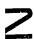
\includegraphics[keepaspectratio]{images/part001_ead1ec0a.jpg}}

Even if \(s \neq \{0\}\) there may exist non-degenerate symmetric bilinear forms on g (Exercise 18 (c)). Such forms, of course, are not associated with any representation of g.

COROLLARY. Let \(\mathfrak{g},\mathfrak{g}'\) be Lie algebras, \(\mathfrak{s}\) (resp. \(\mathfrak{s}'\) ) the nilpotent radical of \(\mathfrak{g}\) (resp. \(\mathfrak{g}'\) ) and \(f\) a homomorphism of \(\mathfrak{g}\) onto \(\mathfrak{g}'\) .

\begin{enumerate}
\def\labelenumi{(\alph{enumi})}
\item
  Then \(\mathfrak{s}' = f(\mathfrak{s})\) .
\item
  \(\mathfrak{g}'\) is reductive if and only if the kernel of \(f\) contains \(\mathfrak{s}\) .
\end{enumerate}

If \(\mathfrak{r},\mathfrak{r}'\) are the radicals of \(\mathfrak{g},\mathfrak{g}',\) then \(\mathfrak{s}' = [\mathfrak{g}',\mathfrak{r}'] = [f(\mathfrak{g}),f(\mathfrak{r})] = f([ \mathfrak{g},\mathfrak{r}]) = f(\mathfrak{s})\) . Assertion (b) is an immediate consequence of (a).

\subsection{APPLICATION: A CRITERION FOR SEMI-SIMPLICITY OF REPRESENTATIONS}

THEOREM 4. Let \(\mathfrak{g}\) be a Lie algebra, \(\mathfrak{r}\) its radical, \(\rho\) a finite-dimensional representation of \(\mathfrak{g},\mathfrak{g}' = \rho (\mathfrak{g})\) and \(\mathfrak{r}' = \rho (\mathfrak{r})\) . Then the following conditions are equivalent:

\begin{enumerate}
\def\labelenumi{(\alph{enumi})}
\item
  \(\rho\) is semi-simple;
\item
  \(\mathfrak{g}'\) is reductive and its centre consists of semi-simple endomorphisms;
\item
  \(\mathfrak{r}'\) consists of semi-simple endomorphisms;
\item
  the restriction of \(\rho\) to \(\mathfrak{r}\) is semi-simple.
\item
  \(\Rightarrow\) (b): if \(\rho\) is semi-simple, \(\mathfrak{g}'\) is reductive (Proposition 5); the associative algebra generated by 1 and \(\mathfrak{g}'\) is semi-simple (Algebra, Chapter VIII, § 5, no. 1, Proposition 3), hence its centre is semi-simple (loc. cit., § 5, no. 4, Proposition 12) and hence the elements of this centre are semi-simple (loc. cit., § 9, no. 1, Proposition 2).
\item
  \(\Rightarrow\) (c): if \(\mathfrak{g}'\) is reductive, its centre is equal to its radical, that is \(\mathfrak{r}'\) , whence the implication (b) \(\Rightarrow\) (c).
\item
  \(\Rightarrow\) (d): suppose that \(\mathfrak{r}'\) consists of semi-simple endomorphisms. As \([\mathfrak{g}',\mathfrak{r}']\) consists of nilpotent endomorphisms (no. 4, Proposition 6), \([\mathfrak{g}',\mathfrak{r}'] = \{0\}\) . Then the implication (c) \(\Rightarrow\) (d) follows from Algebra, Chapter VIII, § 9, no. 2, Theorem 1.
\item
  =\textgreater{} (a): let \(\mathfrak{s}\) be the nilpotent radical of \(\mathfrak{g}\) and \(\rho'\) the restriction of \(\rho\) to \(\mathfrak{r}\) . The elements of \(\rho(\mathfrak{s})\) are nilpotent and hence \(\mathfrak{s}\) is contained in the largest nilpotency ideal of \(\rho'\) . As \(\rho'\) is semi-simple, \(\rho'(\mathfrak{s}) = \{0\}\) and \(\mathfrak{g}'\) is reductive (Corollary to Proposition 6), so that \(\mathfrak{g}' = \mathfrak{a}' \times \mathfrak{r}'\) with \(a'\) semi-simple (Proposition 5). Let \(\mathbf{A}'\) (resp. \(\mathbf{R}'\) ) be the associative algebra generated by 1 and \(a'\) (resp. \(\mathfrak{r}'\) ). It is semi-simple (Algebra, Chapter VIII, § 5, no. 1, Proposition 3), hence \(\mathbf{A}' \otimes_{\mathbb{K}} \mathbf{R}'\) is semi-simple (loc. cit., § 7, no. 6, Corollary 4 to Theorem 3) and hence the associative algebra generated by 1 and \(\mathfrak{g}'\) , which is a quotient of \(\mathbf{A}' \otimes_{\mathbb{K}} \mathbf{R}'\) , is semi-simple, which proves that \(\rho\) is semi-simple.
\end{enumerate}

COROLLARY 1. Let g be a Lie algebra and \(\rho\) and \(\rho'\) two finite-dimensional semi-simple representations of g. Then the tensor product of \(\rho\) and \(\rho'\) is semi-simple.

Let \(\mathfrak{r}\) be the radical of \(\mathfrak{g}\) . For \(x \in \mathfrak{r}\) , \(\rho(x)\) and \(\rho'(x)\) are semi-simple (Theorem 4), hence \(\rho(x) \otimes 1 + 1 \otimes \rho'(x)\) is semi-simple (Algebra, Chapter VIII, § 9, Corollary to Theorem 1) and hence the tensor product of \(\rho\) and \(\rho'\) is semi-simple (Theorem 4).

COROLLARY 2. Let \(\mathfrak{g}\) be a Lie algebra, \(\rho\) a semi-simple representation of \(\mathfrak{g}\) on a finite-dimensional vector space \(V\) , \(T\) and \(S\) the tensor and symmetric algebras of \(V\) and \(\sigma_{T}\) , \(\sigma_{S}\) the representations of \(\mathfrak{g}\) on \(T\) and \(S\) canonically derived from \(\rho\) . Then \(\sigma_{T}\) and \(\sigma_{S}\) are semi-simple and, more precisely, direct sums of finite-dimensional simple representations.

Let \(T^{n}\) be the subspace of T consisting of the homogeneous tensors of order n.~This subspace is stable under \(\sigma_{T}\) and the representation defined by \(\sigma_{T}\) on \(T^{n}\) is semi-simple (Corollary 1). Hence the corollary for \(\sigma_{T}\) and therefore for \(\sigma_{S}\) , which is a quotient representation of \(\sigma_{T}\) .

COROLLARY 3. Let g be a Lie algebra and \(\rho\) and \(\rho'\) two finite-dimensional semi-simple representations of g on spaces M and M'. Then the representation of g on \(\mathcal{L}_{\mathrm{k}}(\mathrm{M},\mathrm{M}')\) canonically derived from \(\rho\) and \(\rho'\) is semi-simple.

The g-module \(\mathcal{L}_{\mathbb{K}}(\mathbf{M},\mathbf{M}^{\prime})\) is canonically identified with the g-module \(\mathbf{M}^{*}\otimes_{\mathbb{K}}\mathbf{M}^{\prime}\) (§ 3, no. 3, Proposition 4), so that Corollary 3 follows from Corollary 1.

COROLLARY 4. Let \(\mathfrak{g}\) be a Lie algebra, a an ideal of \(\mathfrak{g}\) and \(\rho\) a semi-simple representation of \(\mathfrak{g}\) .

\begin{enumerate}
\def\labelenumi{(\alph{enumi})}
\item
  The restriction \(\rho'\) of \(\rho\) to a is semi-simple.
\item
  If \(\rho\) is simple, \(\rho'\) is a sum of simple representations isomorphic to one another.
\end{enumerate}

Passing to the quotient by the kernel of \(\rho\) , \(\rho\) can be assumed to be faithful. Then \(\mathfrak{g}\) is reductive. Let \(\mathfrak{g} = \mathfrak{g}_1 \times \mathfrak{g}_2\) , where \(\mathfrak{g}_1\) is the centre of \(\mathfrak{g}\) and \(\mathfrak{g}_2\) is semi-simple. Then \(\mathfrak{a} = \mathfrak{a}_1 \times \mathfrak{a}_2\) , where \(\mathfrak{a}_1 \subset \mathfrak{g}_1\) , \(\mathfrak{a}_2 \subset \mathfrak{g}_2\) and \(\mathfrak{a}_1\) is the centre of \(\mathfrak{a}\) . The elements of \(\rho(\mathfrak{g}_1)\) , and in particular those of \(\rho(\mathfrak{a}_1)\) , are semi-simple (Theorem 4) and hence \(\rho\) is semi-simple (Theorem 4). Hence (a). Assertion (b) follows from (a), using §3, no. 1, Corollary to Proposition 1.

\subsection{SUBALGEBRAS REDUCTIVE IN A LIE ALGEBRA}

DEFINITION 5. Let g be a Lie algebra and h a Lie subalgebra of g. h is called reductive in g if the representation \(x \mapsto ad_{g} x\) of h is semi-simple.

This representation admits as subrepresentation the adjoint representation of \(\mathfrak{h}\) . Hence, if \(\mathfrak{h}\) is reductive in \(\mathfrak{g},\mathfrak{h}\) is reductive. On the other hand, to say that a Lie algebra is reductive in itself is equivalent to saying that it is reductive.

PROPOSITION 7. Let g be a Lie algebra, h a subalgebra reductive in g, ρ a representation of g on a vector space V and W the sum of the finite-dimensional subspaces of V which are simple h-modules. Then W is stable under ρ(g).

Let \(W_0\) be a finite-dimensional simple sub- \(\mathfrak{h}\) -module of V. We need to prove that \(\rho(x)(W_0) \subset W\) for all \(x \in \mathfrak{g}\) . Let M denote the vector space \(\mathfrak{g}\) considered as an \(\mathfrak{h}\) -module by means of the representation \(x \mapsto \operatorname{ad}_{\mathfrak{g}} x\) of \(\mathfrak{h}\) on \(\mathfrak{g}\) . Then \(M \otimes_{K} W_0\) is a semi-simple \(\mathfrak{h}\) -module (Corollary 1 to Theorem 4). Let \(\theta\) be the K-linear mapping of \(\mathbf{M} \otimes_{\mathbb{K}} \mathbf{W}_0\) into \(\mathbf{V}\) defined by \(\theta(x \otimes w) = \rho(x)w\) . This is an \(\mathfrak{h}\) -module homomorphism, for if \(y \in \mathfrak{h}\) then:

\[
\begin{array}{r l} \theta ([ y, x ] \otimes w + x \otimes \rho (y) w) & = \rho ([ y, x ]) w + \rho (x) \rho (y) w \\ & = \rho (y) \rho (x) w = \rho (y) \theta (x \otimes w). \end{array}
\]

Hence \(\theta (\mathbf{M}\otimes_{\mathbb{K}}\mathbf{W}_0)\) is a finite-dimensional semi-simple \(\mathfrak{h}\) -module. Hence \(\theta (\mathbf{M}\otimes_{\mathbb{K}}\mathbf{W}_0)\subset \mathbf{W}\) , that is \(\rho (x)(\mathbf{W}_0)\subset \mathbf{W}\) for all \(x\in \mathfrak{g}\) .

COROLLARY 1. Let g be a Lie algebra, h a subalgebra reductive in g and \(\rho\) a finite-dimensional semi-simple representation of g. Then the restriction of \(\rho\) to h is semi-simple.

It suffices to consider the case where \(\rho\) is simple. We adopt the notation V, W of Proposition 4. Let \(W_{1}\) be a subspace of V minimal among the nonzero subspaces stable under \(\rho(\mathfrak{h})\) . Then \(W_{1} \subset W\) , hence \(W \neq \{0\}\) and hence \(W = V\) .

COROLLARY 2. Let g be a Lie algebra, h a subalgebra reductive in g and k a subalgebra of h reductive in h. Then k is reductive in g.

The representation \(x \mapsto \operatorname{ad}_{\mathfrak{g}} x\) of \(\mathfrak{h}\) on \(\mathfrak{g}\) is semi-simple and hence its restriction to \(k\) is semi-simple (Corollary 1).

\subsection{EXAMPLES OF SEMI-SIMPLE LIE ALGEBRAS}

PROPOSITION 8. Let V be a finite-dimensional vector space. Then \(\mathfrak{gl}(V)\) is reductive. its centre is the set of homotheties of V, its derived algebra is \(\mathfrak{sl}(V)\) and the latter is semi-simple.

The identity representation of \(\mathfrak{gl}(\mathsf{V})\) is simple, hence \(\mathfrak{gl}(\mathsf{V})\) is reductive and therefore \(\mathfrak{gl}(\mathsf{V})\) is the direct sum of its centre \(c\) and its derived algebra \(\mathcal{D}(\mathfrak{gl}(\mathsf{V}))\) . The centre \(c\) is the set of homotheties (Algebra, Chapter II, §2, no. 5, Corollary 1 to Proposition 5). Clearly \(\mathcal{D}(\mathfrak{gl}(\mathsf{V})) \subset \mathfrak{sl}(\mathsf{V})\) . As \(\mathfrak{sl}(\mathsf{V}) \cap c = \{0\}\) , \(\mathcal{D}(\mathfrak{gl}(\mathsf{V})) = \mathfrak{sl}(\mathsf{V})\) . Hence \(\mathfrak{sl}(\mathsf{V})\) is semi-simple.

Example. We identify \(\mathfrak{sl}(\mathbf{K}^{2})\) with the Lie algebra of matrices of order 2 and trace zero. We write

\[
X = \left( \begin{array}{c c} 0 & 1 \\ 0 & 0 \end{array} \right) \qquad Y = \left( \begin{array}{c c} 0 & 0 \\ 1 & 0 \end{array} \right) \qquad H = \left( \begin{array}{c c} 1 & 0 \\ 0 & - 1 \end{array} \right).
\]

Then \(X, Y, H\) form a basis of \(\mathfrak{sl}(\mathbf{K}^2)\) and

\[
[ H, X ] = 2 X \quad [ H, Y ] = - 2 Y \quad [ X, Y ] = H.
\]

As an algebra of dimension 1 or 2 is not semi-simple (no. 1, Remark 1), \(\mathfrak{sl}(\mathbf{K}^2)\) is simple. In fact, \(\mathfrak{sl}(\mathbf{V})\) is simple for \(\dim V \geqslant 2\) , as we shall see later (cf.~also Exercises 21 and 24).

PROPOSITION 9. Let \(\mathrm{V}\) be a vector space of finite dimension \(n\) over \(\mathbf{K}\) and \(\beta\) a nondegenerate symmetric (resp. alternating) bilinear form on \(\mathrm{V}\) . Let \(\mathfrak{g}\) be the Lie algebra consisting of the \(x \in \mathfrak{gl}(\mathrm{V})\) such that \(\beta (xm, m') + \beta (m, xm') = 0\) for all \(m, m'\) in \(\mathrm{V}\) . Then \(\mathfrak{g}\) is reductive; \(\mathfrak{g}\) is even semi-simple except in the case where \(\beta\) is symmetric and \(n = 2\) .

For all \(u \in \mathfrak{gl}(\mathrm{V})\) let \(u^*\) denote its adjoint relative to \(\beta\) ; then \(\operatorname{Tr}(u) = \operatorname{Tr}(u^*)\) by Proposition 7 of Algebra, Chapter IX, § 1, no. 8. The condition

\[
\beta (u m, m ^ {\prime}) + \beta (m, u m ^ {\prime}) = 0
\]

for all \(m\) , \(m'\) in V means that \(u + u^{*} = 0\) . In particular, if \(v \in \mathfrak{gl}(V)\) then \((v - v^{*})^{*} = v^{*} - v\) and hence \(v - v^{*} \in \mathfrak{g}\) . Then let \(u\) be an element of \(\mathfrak{g}\) orthogonal to \(\mathfrak{g}\) with respect to the bilinear form \(\phi\) associated with the identity representation of \(\mathfrak{g}\) . For all \(v \in \mathfrak{gl}(V)\) , \(\operatorname{Tr} u(v - v^{*}) = 0\) , hence

\[
\operatorname{Tr} (u v) = \operatorname{Tr} (u v ^ {*}) = \operatorname{Tr} (u v ^ {*}) ^ {*} = \operatorname{Tr} (v u ^ {*}) = - \operatorname{Tr} (v u) = - \operatorname{Tr} (u v)
\]

and hence \(\operatorname{Tr}(u v) = 0\) . It follows that \(u = 0\) , so that \(\phi\) is non-degenerate. Hence \(\mathfrak{g}\) is reductive (Proposition 5). It remains to show that the centre of \(\mathfrak{g}\) is zero (except when \(\beta\) is symmetric and \(n = 2\) ). By extending the base field, we can assume that \(\mathbf{K}\) is algebraically closed.

\begin{enumerate}
\def\labelenumi{(\alph{enumi})}
\item
  When \(\beta\) is symmetric, it can be identified with the bilinear form on \(\mathbf{K}^n\) with matrix \(I_{\mathrm{n}}\) with respect to the canonical basis (Algebra, Chapter IX, §6, Corollary 1 to Theorem 1). Under these conditions \(\mathfrak{g}\) is identified with the Lie algebra of skew-symmetric matrices (§3, no. 4, Example 1). Let \(U = (u_{ij}) \in \mathfrak{g}\) ; we use the fact that \(U\) commutes with the matrix \((v_{ij}) \in \mathfrak{g}\) all of whose elements are zero except \(v_{i_0j_0}\) and \(v_{j_0i_0}\) ( \(i_0 \neq j_0\) ) which are equal respectively to 1 and -1. We find that \(u_{i_0j} = u_{j_0j} = u_{ii_0} = u_{ij_0} = 0\) for \(i \neq i_0, j_0\) and \(j \neq i_0, j_0\) . If \(n > 2\) , there exist, for all distinct indices \(i_0\) and \(j\) , distinct indices \(i\) and \(j_0\) such that \(i \neq i_0, j_0 \neq j, j_0 \neq i_0\) ; hence \(u_{i_0j} = 0\) . This proves that an element of the centre of \(\mathfrak{g}\) is zero.
\item
  When \(\beta\) is alternating and \(n = 2m\) , \(\beta\) can be identified with the bilinear form on \(\mathbf{K}^{2m}\) with matrix \(\left( \begin{array}{cc}0 & I_m \\ -I_m & 0 \end{array} \right)\) with respect to the canonical basis (Algebra, Chapter IX, §5, Corollary 1 to Theorem 1). Under these conditions \(\mathfrak{g}\) is identified with the Lie algebra of matrices of the form \(U = \left( \begin{array}{cc}A & B\\ C & D \end{array} \right)\) where \(D = -^t A\) , \(B\) and \(C\) are symmetric ( \(A, B, C, D\) in \(\mathbf{M}_m(\mathbf{K})\) ) (§3, no. 4, Example 1). We use first the fact that \(U\) commutes with the matrix \(\left( \begin{array}{cc}X & 0 \\ 0 & -^t X \end{array} \right)\) , where \(X \in \mathbf{M}_m(\mathbf{K})\) . Then \(AX = X A\) , \(CX = -^t XC\) , \(XB = -B\) . \(^t X\) ; as these equalities must hold for all \(X\) , it follows that \(A\) is a scalar matrix \(\lambda I_m\) . We now use the fact that \(U\) commutes with the matrix \(\left( \begin{array}{cc}0 & Y \\ 0 & 0 \end{array} \right)\) , where
\end{enumerate}

\(Y\) is a symmetric matrix of \(\mathbf{M}_m(\mathrm{K})\) . Then \(\lambda Y = YC = CY = 0\) . This proves first that \(\lambda = 0\) . Moreover, for all \(X \in \mathbf{M}_m(\mathrm{K})\) , \(X + {}^t X\) is symmetric and hence \(XC = -{}^t XC\) . Using the equation \(CX = -{}^t XC\) obtained above, we see that \(C\) commutes with every element of \(\mathbf{M}_m(\mathrm{K})\) and hence that \(C\) is a scalar matrix, necessarily zero since \(YC = 0\) . It is similarly shown that \(B = 0\) .

For \(\beta\) symmetric and \(n = 2\) , \(\mathfrak{g}\) is of dimension 1 and hence commutative. For the other cases cf.~Exercises 25 and 26.

\subsection{THE LEVI-MALCEV THEOREM}

Let E be a complete normed vector space over R and u a continuous endomorphism of E. We have seen (Functions of a real variable, Chapter IV, § 2, no. 6) that the sequence \(\frac{u^{n}}{n!}\) is summable in \(\mathcal{L}(E)\) and we wrote

\[
e ^ {u} = \exp u = \sum_ {n = 0} ^ {\infty} \frac {u ^ {n}}{n !}.
\]

Now let E be a vector space over the field K and u a nilpotent endomorphism of E. The series \(\sum_{n=0}^{\infty}\frac{u^{n}}{n!}\) has only a finite number of non-zero terms and we can therefore write

\[
e ^ {u} = \exp u = \sum_ {n = 0} ^ {\infty} \frac {u ^ {n}}{n !}.
\]

This definition agrees with the above if K = R and if E is complete and normed. If v is another nilpotent endomorphism of E which commutes with u, then:

\[
\begin{array}{l} e ^ {u} e ^ {v} = \left(\sum_ {n = 0} ^ {\infty} \frac {u ^ {n}}{n !}\right) \left(\sum_ {p = 0} ^ {\infty} \frac {v ^ {p}}{p !}\right) = \sum_ {n, p = 0} ^ {\infty} \frac {u ^ {n} v ^ {p}}{n ! p !} \\ = \sum_ {q = 0} ^ {\infty} \frac {1}{q !} \left(\sum_ {n + p = q} \binom {q} {n} u ^ {n} v ^ {p}\right) = \sum_ {q = 0} ^ {\infty} \frac {1}{q !} (u + v) ^ {q} = e ^ {u + v}. \end{array}\tag{3}
\]

In particular, \(e^u e^{-u} = e^{-u}e^u = e^0 = 1\) and hence \(e^u\) is always an automorphism of E.

If further E is a (not necessarily associative) algebra and u is a (nilpotent) derivation of E, then \(e^{u}\) is an automorphism of the algebra E. For if \(x, y \in E\) then

\[
u ^ {p} (x y) = \sum_ {r + s = p} \binom {p} {r} u ^ {r} (x) u ^ {s} (y)
\]

for every integer \(p \geqslant 0\) (Leibniz's formula). It follows that

\[
\begin{array}{r l} e ^ {u} (x y) & = \sum_ {p \geqslant 0} \frac {1}{p !} u ^ {p} (x y) = \sum_ {p \geqslant 0} \sum_ {r + s = p} \frac {u ^ {r} (x)}{r !} \frac {u ^ {s} (y)}{s !} \\ & = \sum_ {r, s = 0} ^ {\infty} \frac {u ^ {r} (x)}{r !} \frac {u ^ {s} (y)}{s !} = e ^ {u} (x) e ^ {u} (y) \end{array}
\]

whence our assertion.

Now let g be a Lie algebra. If x belongs to the nilpotent radical of g, the derivation \(ad_{g}x\) of g is nilpotent. We can therefore make the following definition:

DEFINITION 6. A special automorphism of g is an automorphism of g of the form \(e^{ad_{\mathfrak{g}} x}\) , where x is in the nilpotent radical of g.

Clearly a special automorphism leaves every ideal of g stable.

DEFINITION 7. Let \(\mathfrak{g}\) be a Lie algebra and \(\mathfrak{r}\) its radical. A Levi subalgebra of \(\mathfrak{g}\) is any subalgebra of \(\mathfrak{g}\) supplementary to \(\mathfrak{r}\) .

A Levi subalgebra is isomorphic to \(\mathfrak{g} / \mathfrak{r}\) and hence is semi-simple. As a semi-simple subalgebra has only 0 in common with \(\mathfrak{r}\) , every semi-simple subalgebra \(\mathfrak{h}\) such that \(\mathfrak{g} = \mathfrak{r} + \mathfrak{h}\) is a Levi subalgebra; consequently the image of a Levi subalgebra under a surjective homomorphism is a Levi subalgebra.

THEOREM 5 (Levi--Malcev). A Lie algebra g always has a Levi subalgebra s. Every Levi subalgebra of g is the image of s under a special automorphism.

Let r denote the radical of g. We first treat two special cases.

\begin{enumerate}
\def\labelenumi{(\alph{enumi})}
\tightlist
\item
  \([g, r] = \{0\}\) .
\end{enumerate}

By Proposition 5, g is then the product of its centre r by Dg which is semi-simple. Hence Dg is a Levi subalgebra. Moreover, if \(s'\) is a semi-simple subalgebra, then \(s' = Ds'\) (Theorem 1), hence \(s' \subset Dg\) and Dg is the unique Levi subalgebra of g.

\begin{enumerate}
\def\labelenumi{(\alph{enumi})}
\setcounter{enumi}{1}
\tightlist
\item
  \([\mathfrak{g},\mathfrak{r}]\neq \{0\}\) and the only ideals of \(\mathfrak{g}\) contained in \(\mathfrak{r}\) are \(\{0\}\) and \(\mathfrak{r}\) .
\end{enumerate}

Then \([\mathfrak{g},\mathfrak{r}] = \mathfrak{r}\) , \([\mathfrak{r},\mathfrak{r}] = \{0\}\) and the centre of \(\mathfrak{g}\) is zero. Let M (resp. N) be the subspace of \(\mathcal{L}(\mathfrak{g})\) consisting of the linear mappings of \(\mathfrak{g}\) into \(\mathfrak{r}\) whose restriction to \(\mathfrak{r}\) is a homothety (resp. zero); N is therefore of codimension 1 in M. For \(m\in M\) , let \(\lambda (m)\) denote the ratio of the homothety of \(\mathfrak{r}\) defined by \(m\) . Let \(\sigma\) be the representation of \(\mathfrak{g}\) on \(\mathcal{L}(\mathfrak{g})\) canonically derived from the adjoint representation; recall that \(\sigma (x).u = [\mathrm{ad}_{\mathfrak{g}}x,u]\) for all \(x\in \mathfrak{g}\) and all \(u\in \mathcal{L}(\mathfrak{g})\) .

\[
\mathcal{L}(\mathfrak{g}) \supset \mathrm{M} \supset \mathrm{N} \supset \mathrm{P}
\]
Clearly \(\sigma (x)(\mathrm{M})\subset \mathrm{N}\) for all \(x\in \mathfrak{g}\) . Moreover, if \(x\in \mathfrak{r},y\in \mathfrak{g}\) and \(u\in \mathrm{M}\) , then\\
(4) \((\sigma (x).u)(y) = [x,u(y)] - u([x,y]) = -\lambda (u)[x,y]\) since \([\mathfrak{r},\mathfrak{r}] = \{0\}\) ; and (4) can be written:\\
(5) \(\sigma (x).u = -\mathrm{ad}(\lambda (u).x)\) .

As the centre of g is zero, the mapping \(x \mapsto ad_{g}x\) defines a bijection \(\phi\) of r onto a subspace P of \(\mathcal{L}(\mathfrak{g})\) . This subspace is stable under \(\sigma(\mathfrak{g})\) and contained in N since r is a commutative ideal and (5) shows that \(\sigma(x)(\mathrm{M}) \subset \mathrm{P}\) for \(x \in \mathfrak{r}\) . The representation of g on M/P = V derived from \(\sigma\) is therefore zero on r and defines a representation \(\sigma'\) of the semi-simple algebra g/r on V. For all \(y \in g/r\) , the space \(\sigma'(y)(V)\) is contained in N/P, which is of codimension 1 in V. Consequently (no. 2, Lemma 3) there exists \(u_{0} \in M\) such that \(\lambda(u_{0}) = -1\) and \(\sigma(x).u_{0} \in P\) for all \(x \in g\) . The mapping \(x \mapsto \phi^{-1}(\sigma(x).u_{0})\) is a linear mapping of g into r. By (5) its restriction to r is the identity mapping of r. Hence its kernel is a subspace s of g supplementary to r in g. As s is the set of \(x \in g\) such that \(\sigma(x).u_{0} = 0\) , s is a subalgebra of g and therefore a Levi subalgebra of g.

Let \(\mathfrak{s}'\) be another Levi subalgebra. For all \(x \in \mathfrak{s}'\) , let \(h(x)\) be the unique element of \(\mathfrak{r}\) such that \(x + h(x) \in \mathfrak{s}\) . Since \(\mathfrak{s}\) is a subalgebra and \(\mathfrak{r}\) is commutative, for \(x, y\) in \(\mathfrak{s}'\) :

\[
[ x + h (x), y + h (y) ] = [ x, y ] + [ x, h (y) ] + [ h (x), y ] \in \mathfrak {s}
\]

hence

\[
h ([ x, y ]) = (\operatorname{ad} x). h (y) - (\operatorname{ad} y). h (x).
\]

By Remark 2 of no. 2, there exists \(a \in \mathfrak{r}\) such that \(h(x) = -[x, a]\) for all \(x \in \mathfrak{s}'\) . Then:

\[
x + h (x) = x + [ a, x ] = (1 + \operatorname{ad} a). x.\tag{6}
\]

As \(\mathfrak{r}\) is commutative, \((\operatorname{ad} a)^2 = 0\) and hence \(1 + \operatorname{ad} a = e^{\operatorname{ad} a}\) . As \(\mathfrak{r} = [\mathfrak{s}, \mathfrak{r}]\) , \(e^{\operatorname{ad} a}\) is a special automorphism of \(\mathfrak{g}\) . By (6) this special automorphism maps \(\mathfrak{s}'\) to \(\mathfrak{s}\) .

\textbf{(c) General case:}

We argue by induction on the dimension \(n\) of the radical. There is nothing to prove if \(n = 0\) and hence it can be assumed that the theorem holds for Lie algebras whose radical is of dimension \(<\dim \mathfrak{r}\) . By (a) it suffices to consider the case where \([\mathfrak{g}, \mathfrak{r}] \neq \{0\}\) . As \([\mathfrak{g}, \mathfrak{r}]\) is nilpotent (no. 4, Proposition 6), its centre \(\mathfrak{c}\) is \(\neq \{0\}\) . Let \(\mathfrak{m}\) be a minimal non-zero ideal of \(\mathfrak{g}\) contained in \(\mathfrak{c}\) . If \(\mathfrak{m} = \mathfrak{r}\) , we have case (b). Therefore let \(\mathfrak{m} \neq \mathfrak{r}\) and let \(f\) be the canonical mapping of \(\mathfrak{g}\) onto \(\mathfrak{g}' = \mathfrak{g}/\mathfrak{m}\) . The radical of \(\mathfrak{g}'\) is \(\mathfrak{r}' = \mathfrak{r}/\mathfrak{m}\) . By the induction hypothesis, \(\mathfrak{g}'\) has a Levi subalgebra \(\mathfrak{h}'\) . Then \(\mathfrak{h} = f^{-1}(\mathfrak{h}')\) is a subalgebra of \(\mathfrak{g}\) containing \(\mathfrak{m}\) such that \(\mathfrak{h}/\mathfrak{m} = \mathfrak{h}'\) is semi-simple and hence having \(\mathfrak{m}\) as radical. By the induction hypothesis \(\mathfrak{h} = \mathfrak{m} + \mathfrak{s}\) where \(\mathfrak{s}\) is a semi-simple subalgebra. Then the equality \(\mathfrak{g}' = \mathfrak{r}' + \mathfrak{h}'\) implies \(\mathfrak{g} = \mathfrak{r} + \mathfrak{h} = \mathfrak{r} + \mathfrak{m} + \mathfrak{s} = \mathfrak{r} + \mathfrak{s}\) and hence \(\mathfrak{s}\) is a Levi subalgebra of \(\mathfrak{g}\).

Let \(\mathfrak{s}'\) be another Levi subalgebra of \(\mathfrak{g}\) . Then \(f(\mathfrak{s})\) and \(f(\mathfrak{s}')\) are two Levi subalgebras of \(\mathfrak{g}'\) and there exists by the induction hypothesis \(a' \in [\mathfrak{g}', \mathfrak{r}']\) such that \(e^{\mathrm{ad} a'}(f(\mathfrak{s}')) = f(\mathfrak{s})\) . If \(a \in [\mathfrak{g}, \mathfrak{r}]\) is such that \(f(a) = a'\) , it follows that:

\[
\mathfrak {s} _ {1} = e ^ {\mathrm{ad} a} \left(\mathfrak {s} ^ {\prime}\right) \subset \mathfrak {m} + \mathfrak {s} = \mathfrak {h}.
\]

Then \(\mathfrak{s}_1\) and \(\mathfrak{s}\) are two Levi subalgebras of \(\mathfrak{h}\) and by the induction hypothesis there exists \(b\in \mathfrak{m}\) such that \(e^{\mathrm{ad}b}(\mathfrak{s}_1) = \mathfrak{s}\) . Hence \(\mathfrak{s} = e^{\mathrm{ad}b}.e^{\mathrm{ad}a}(\mathfrak{s}')\) . Finally, as \(\mathfrak{m}\) is in the centre of \([\mathfrak{g},\mathfrak{r}]\) , \(e^{\mathrm{ad}b}.e^{\mathrm{ad}a} = e^{\mathrm{ad}(b + a)}\) and \(b + a\in [\mathfrak{g},\mathfrak{r}]\) , which completes the proof.

COROLLARY 1. Let \(\mathfrak{s}\) be a Levi subalgebra of \(\mathfrak{g}\) and \(\mathfrak{h}\) a semi-simple subalgebra of \(\mathfrak{g}\) .

\begin{enumerate}
\def\labelenumi{(\alph{enumi})}
\item
  There exists a special automorphism of \(\mathfrak{g}\) mapping \(\mathfrak{h}\) onto a subalgebra of \(\mathfrak{s}\) .
\item
  \(\mathfrak{h}\) is contained in a Levi subalgebra of \(\mathfrak{g}\) .
\end{enumerate}

Let \(\mathfrak{r}\) be the radical of \(\mathfrak{g}\) and \(\mathfrak{a} = \mathfrak{h} + \mathfrak{r}\) , which is a subalgebra of \(\mathfrak{g}\) . Then \(\mathfrak{a}/\mathfrak{r}\) is semi-simple and \(\mathfrak{r}\) is solvable, hence \(\mathfrak{r}\) is the radical of \(\mathfrak{a}\) and \(\mathfrak{h}\) is a Levi subalgebra of \(\mathfrak{a}\) . On the other hand, \(\mathfrak{a} \cap \mathfrak{s} = \mathfrak{h}'\) is a supplementary subalgebra to \(\mathfrak{r}\) in \(\mathfrak{a}\) and hence also a Levi subalgebra of \(\mathfrak{a}\) . Then there exists (Theorem 5) \(a \in [\mathfrak{a}, \mathfrak{r}]\) such that \(e^{\mathrm{ad} a}\) maps \(\mathfrak{h}\) onto \(\mathfrak{h}'\) . Now \(a \in [\mathfrak{g}, \mathfrak{r}]\) ; \(e^{\mathrm{ad} a}\) maps \(\mathfrak{h}\) onto a subalgebra of \(\mathfrak{s}\) and \(e^{-\mathrm{ad} a}(\mathfrak{s})\) is a Levi subalgebra of \(\mathfrak{g}\) containing \(\mathfrak{h}\) .

COROLLARY 2. For a subalgebra \(\mathfrak{h}\) of \(\mathfrak{g}\) to be a Levi subalgebra of \(\mathfrak{g}\) , it is necessary and sufficient that \(\mathfrak{h}\) be a maximal semi-simple subalgebra of \(\mathfrak{g}\) .

This follows immediately from Corollary 1.

COROLLARY 3. Let g be a Lie algebra and m an ideal of g such that g/m is semi-simple. Then g contains a subalgebra supplementary to m in g. In other words, every extension of a semi-simple Lie algebra is inessential.

Let \(\mathfrak{s}\) be a Levi subalgebra of \(\mathfrak{g}\) (Theorem 5). Its canonical image in \(\mathfrak{g}/\mathfrak{m}\) is a Levi subalgebra and therefore equal to \(\mathfrak{g}/\mathfrak{m}\) , hence \(\mathfrak{g} = \mathfrak{s} + \mathfrak{m}\) . Then an ideal of \(\mathfrak{s}\) supplementary in \(\mathfrak{s}\) to the ideal \(\mathfrak{m} \cap \mathfrak{s}\) is a subalgebra of \(\mathfrak{g}\) supplementary to \(\mathfrak{m}\) in \(\mathfrak{g}\) .

COROLLARY 4. Let g be a Lie algebra, r its radical, s a Levi subalgebra of g and m an ideal of g. Then m is the direct sum of m ∩ r which is its radical and m ∩ s which is a Levi subalgebra of m.

We know that \(\mathfrak{m} \cap \mathfrak{s}\) is the radical of \(\mathfrak{m}\) (§ 5, no. 5, Corollary 3 to Proposition 5). Let \(\mathfrak{h}\) be a Levi subalgebra of \(\mathfrak{m}\) and \(\mathfrak{s}'\) a Levi subalgebra of \(\mathfrak{g}\) containing \(\mathfrak{h}\) (Corollary 1). The algebra \(\mathfrak{m} \cap \mathfrak{s}'\) is an ideal of \(\mathfrak{s}'\) , is therefore semi-simple, and contains \(\mathfrak{h}\) and is therefore equal to \(\mathfrak{h}\) . Hence \(\mathfrak{m}\) is the direct sum of \(\mathfrak{m} \cap \mathfrak{r}\) and \(\mathfrak{m} \cap \mathfrak{s}'\) . There exists a special automorphism mapping \(\mathfrak{s}'\) onto \(\mathfrak{s}\) ; this automorphism leaves \(\mathfrak{r}\) and \(\mathfrak{m}\) invariant; hence \(\mathfrak{m}\) is the direct sum of \(\mathfrak{m} \cap \mathfrak{r}\) and \(\mathfrak{m} \cap \mathfrak{s}\) and \(\mathfrak{m} \cap \mathfrak{s}\) is a Levi subalgebra of \(\mathfrak{m}\) .

\subsection{THE INVARIANTS THEOREM}

Let g be a Lie algebra and \(\rho\) a representation of g on a vector space M. For every class \(\delta\) of simple representations of g let \(M_{\delta}\) be the isotypical component of M of species \(\delta\) . The subspace \(M_{0}\) of invariant elements of M is just \(M_{\delta_{0}}\) , where \(\delta_{0}\) denotes the class of the zero representation of g on a space of dimension 1.

Lemma 4. Let \(\rho, \sigma, \tau\) be representations of \(\mathfrak{g}\) on vector spaces \(\mathbf{M}, \mathbf{N}, \mathbf{P}\) . Suppose that we are given a K-bilinear mapping \((m, n) \mapsto m \cdot n\) of \(\mathbf{M} \times \mathbf{N}\) into \(\mathbf{P}\) such that

\[
(\rho (x) m). n + m. (\sigma (x) n) = \tau (x) (m. n)
\]

for all \(m \in M\) , \(n \in N\) , \(x \in g\) .

\begin{enumerate}
\def\labelenumi{(\alph{enumi})}
\item
  If \(m_0 \in \mathbf{M}_0\) , the mapping \(n \mapsto m_0\) . \(n\) is a \(\mathfrak{g}\) -module homomorphism.
\item
  If \(n \in N_{\delta}\) , then \(m_{0}.n \in P_{\delta}\) .
\item
  If \(\mathbf{M}\) is a (not necessarily associative) algebra and the \(\rho(x)\) are derivations of \(\mathbf{M}\) , \(\mathbf{M}_0\) is a subalgebra of \(\mathbf{M}\) and each \(\mathbf{M}_{\delta}\) is a right and left \(\mathbf{M}_0\) -module.
\end{enumerate}

For \(m_{0} \in M_{0}, n \in N\) and \(x \in g,\)

\[
\tau (x) \left(m _ {0}. n\right) = m _ {0}. (\sigma (x) n),
\]

whence (a). Assertion (b) follows from (a) (Algebra, Chapter VIII, § 3, no. 4, Proposition 10). If \(\mathbf{N} = \mathbf{P} = \mathbf{M}\) and \(\sigma = \tau = \rho\) , assertion (b) gives assertion (c) as a special case.

Lemma 5. Suppose further that \(\sigma\) and \(\tau\) are semi-simple and hence N (resp. P) is the direct sum of the \(N_{\delta}\) (resp. \(P_{\delta}\) ). For all \(n \in N\) (resp. \(p \in P\) ), let \(n^{\sharp}\) (resp. \(p^{\sharp}\) ) be its component in \(N_0\) (resp. \(P_0\) ). Let \(m_0 \in M_0\) . Then for all \(n \in N\) , \((m_0.n)^{\sharp} = m_0.n^{\sharp}\) .

By linearity it suffices to consider the case where \(n \in \mathrm{N}_{\delta}\) . If \(\delta \neq \delta_0\) , \(n^{\sharp} = 0\) and \(m_0.n \in \mathrm{P}_{\delta}\) (Lemma 4), hence \((m_0.n)^{\sharp} = 0 = m_0.n^{\sharp}\) . If \(\delta = \delta_0\) , \(n^{\sharp} = n\) and \(m_0.n \in \mathrm{P}_0\) (Lemma 4), hence \((m_0.n)^{\sharp} = m_0.n = m_0.n^{\sharp}\) .

THEOREM 6. Let \(\mathfrak{g}\) be a Lie algebra, V a semi-simple \(\mathfrak{g}\) -module of finite dimension over K, S the symmetric algebra of V and \(x_{\mathrm{S}}\) the derivation of S which extends \(x_{\mathrm{V}}\) (so that \(x \mapsto x_{\mathrm{S}}\) is a representation of \(\mathfrak{g}\) on S).

\begin{enumerate}
\def\labelenumi{(\alph{enumi})}
\item
  The algebra \(\mathbf{S}_0\) of invariants of \(\mathbf{S}\) is generated by a finite number of elements.
\item
  For every class \(\delta\) of simple representations of \(\mathfrak{g}\) of finite dimension over \(\mathbf{K}\) , let \(\mathrm{S}_{\delta}\) be the isotypical component of \(\mathrm{S}\) of species \(\delta\) . Then \(\mathrm{S}_{\delta}\) is a finitely generated \(\mathrm{S}_{0}\) -module.
\end{enumerate}

Let \(\overline{\mathbf{S}}\subset \mathbf{S}\) be the ideal of elements of S with no constant term. Let I be the ideal of S generated by \(\mathrm{S}_0\cap \overline{\mathrm{S}}\) and let \((s_1,s_2,\ldots ,s_p)\) be a finite system of generators of the ideal I (Commutative Algebra, Chapter III, § 3). It can be assumed that the \(s_t\) belong to \(\mathbf{S}_0 \cap \bar{\mathbf{S}}\) and are homogeneous (the \(x_{\mathrm{S}}\) preserve degrees and hence each \(\mathbf{S}_0\) is a graded submodule). Let \(\mathbf{S}_1\) be the subalgebra of \(\mathbf{S}\) generated by 1 and the \(s_t\) . Then \(\mathbf{S}_1 \subset \mathbf{S}_0\) . We show that \(\mathbf{S}_1 = \mathbf{S}_0\) . For this we prove that every homogeneous element \(s\) of \(\mathbf{S}_0\) is in \(\mathbf{S}_1\) , arguing by induction on the degree \(n\) of \(s\) . If \(n = 0\) , our assertion is obvious. Suppose therefore \(n > 0\) and that our assertion has been proved when the degree of s is \(< n\) . As \(s \in I\) , \(s = \sum_{i=1}^{p} s_i s_i'\) , where the \(s_i'\) are elements of S which can be assumed to be homogeneous, with \(\deg(s_i') = \deg(s) - \deg(s_i) < n\) . Lemma 5 can be applied, as the g-module S is semi-simple (no. 5, Corollary 2 to Theorem 4); in the notation of this lemma,

\[
s = s ^ {\sharp} = \sum_ {i = 1} ^ {p} (s _ {i} s _ {i} ^ {\prime}) ^ {\sharp} = \sum_ {i = 1} ^ {p} s _ {i} {s _ {i} ^ {\prime}} ^ {\sharp}.
\]

The \(s_i^\sharp\) are elements of \(S_0\) which are homogeneous and of degree \(< n\) (since each \(S_\delta\) is a graded submodule). Hence they are in \(S_1\) by the induction hypothesis. Hence \(s \in S_1\) , which proves (a).

We now consider a simple representation of g of class \(\delta\) on a finite-dimensional space M. Let \(L = \mathcal{L}_{\mathbb{K}}(M, S)\) . For all \(s \in S\) and all \(f \in L\) , let sf be the element of L defined by \((sf)(m) = s.f(m)\) ( \(m \in M\) ); an S-module structure is thus defined on L; as M is finite-dimensional over K, clearly L is a finitely generated S-module and hence a Noetherian S-module since the ring S is Noetherian. On the other hand, L has a canonical g-module structure. For every integer \(n \geqslant 0\) let \(S^{n}\) be the set of homogeneous elements of S of degree n; then the g-module \(\mathcal{L}_{\mathbb{K}}(M, S^{n})\) is semi-simple (no. 5, Corollary 3 to Theorem 4) and hence the g-module L is semi-simple. Moreover, for \(s \in S\) , \(f \in L\) , \(x \in g\) and \(m \in M\) ,

\[
\begin{array}{r l} (x _ {\mathrm{L}} (s f)) (m) & = x _ {\mathrm{S}} ((s f) (m)) - (s f) (x _ {\mathrm{M}} m) \\ & = x _ {\mathrm{S}} (s. f (m)) - s. f (x _ {\mathrm{M}} m) \\ & = (x _ {\mathrm{S}} s). f (m) + s. (x _ {\mathrm{S}} f (m)) - s. f (x _ {\mathrm{M}} m) \\ & = ((x _ {\mathrm{S}} s) f) (m) + (s (x _ {\mathrm{L}} f)) (m) \end{array}
\]

and hence \(x_{\mathrm{L}}(sf) = (x_{\mathrm{S}}s)f + s(x_{\mathrm{L}}f)\) . We can therefore apply Lemma 5.

The subset \(\mathbf{L}_0\) of invariant elements of \(\mathbf{L}\) is just the set of homomorphisms of the \(g\) -module \(\mathbf{M}\) into the \(g\) -module \(\mathbf{S}\) . Hence, if \(\phi\) denotes the canonical homomorphism of \(\mathrm{M} \otimes_{\mathrm{K}} \mathrm{L}\) onto \(\mathrm{S}\) , \(\phi(\mathrm{M} \otimes_{\mathrm{K}} \mathrm{L}_0) = \mathrm{S}_{\delta}\) . As \(\phi\) is obviously an S-module homomorphism, it suffices to show that \(\mathbf{L}_0\) is a finitely generated \(\mathrm{S}_0\) -module. Let \(\mathbf{J}\) be the sub-S-module of \(\mathbf{L}\) generated by \(\mathbf{L}_0\) . Since \(\mathbf{L}\) is a Noetherian S-module, there exists a finite sequence \((f_1, \ldots, f_q)\) of elements of \(\mathbf{L}_0\) generating the S-module \(\mathbf{J}\) . Let \(\mathbf{L}_1\) be the \(\mathrm{S}_0\) -module generated by \(f_{1},\ldots ,f_{q}\) . Then \(\mathrm{L}_1\subset \mathrm{L}_0\) . On the other hand, if \(f\in \mathrm{L}_0\) , then \(f = \sum_{i = 1}^{q}s_{i},f_{i}\) with \(s_i\in S\) for all \(i\) and hence by Lemma 5 whose notation we adopt:

\[
f = f ^ {\sharp} = \left(\sum_ {i = 1} ^ {q} s _ {i} f _ {i}\right) ^ {\sharp} = \sum_ {i = 1} ^ {q} s _ {i} ^ {\sharp} f _ {i} \in L _ {1}.
\]

Hence \(L_{0} = L_{1}\) , so that \(L_{0}\) is a finite generated \(S_{0}\) -module.

\subsection{CHANGE OF BASE FIELD}

Let \(K_{1}\) be a commutative extension of K. For a Lie algebra g over K to be semi-simple, it is necessary and sufficient that \(g_{(K_{1})}\) be semi-simple; for the Killing form \(\beta_{1}\) of \(g_{(K_{1})}\) is derived from the Killing form \(\beta\) of g by extending the base field from K to \(K_{1}\) ; hence \(\beta_{1}\) is non-degenerate if and only if \(\beta\) is non-degenerate (Algebra, Chapter IX, § 1, no. 4, Corollary to Proposition 3).

If \(\mathfrak{g}_{(\mathbf{K}_{1})}\) is simple, g is semi-simple by the above and cannot be a product of two non-zero ideals, hence g is simple. On the other hand if g is simple \(\mathfrak{g}_{(\mathbf{K}_{1})}\) (which is semi-simple) may be not simple (Exercises 17 and 26 (b)).

Let \(\mathfrak{g}\) be a Lie algebra and \(\mathfrak{r}\) its radical. Then \(\mathfrak{r}_{(\mathbf{K}_1)}\) is the radical of \(\mathfrak{g}_{(\mathbf{K}_1)}\) (§ 5, no. 6). Therefore, if \(\mathfrak{s}\) denotes the nilpotent radical of \(\mathfrak{g}\) , the nilpotent radical of \(\mathfrak{g}_{(\mathbf{K}_1)}\) is \([\mathfrak{g}_{(\mathbf{K}_1)},\mathfrak{r}_{(\mathbf{K}_1)}] = [\mathfrak{g},\mathfrak{r}]_{(\mathbf{K}_1)} = \mathfrak{s}_{(\mathbf{K}_1)}\) . It follows that \(\mathfrak{g}\) is reductive if and only if \(\mathfrak{g}_{(\mathbf{K}_1)}\) is reductive.

Let \(\mathfrak{g}\) be a Lie algebra and \(\mathfrak{h}\) a subalgebra. Recall that a representation of \(\mathfrak{h}\) is semi-simple if and only if the representation of \(\mathfrak{h}_{(\mathrm{K}_1)}\) derived by extending the base field to \(\mathrm{K}_1\) is semi-simple. Hence \(\mathfrak{h}\) is reductive in \(\mathfrak{g}\) if and only if \(\mathfrak{h}_{(\mathrm{K}_1)}\) is reductive in \(\mathfrak{g}_{(\mathrm{K}_1)}\) .

Now let \(K_{0}\) be a subfield of K such that \([K:K_{0}]\) is finite. Let g be a Lie algebra and \(g_{0}\) the (finite-dimensional) Lie algebra derived from g by restricting the base field from K to \(K_{0}\) . Every commutative ideal of g is a commutative ideal of \(g_{0}\) ; conversely, if \(a_{0}\) is a commutative ideal of \(g_{0}\) the smallest vector subspace over K of g containing \(a_{0}\) is a commutative ideal of g; hence g is semi-simple if and only if \(g_{0}\) is semi-simple. If \(g_{0}\) is simple, clearly g is simple. Conversely, suppose that g is simple. We show that \(g_{0}\) is simple. Let \(a_{0}\) be a simple component of \(g_{0}\) . For all \(\lambda \in K^{*}\) , \(\lambda a_{0}\) is an ideal of \(g_{0}\) and

\[
\left[ a _ {0}, \lambda a _ {0} \right] = \lambda \left[ a _ {0}, a _ {0} \right] = \lambda a _ {0} \neq \{0 \},
\]

hence \(\lambda a_0 \supset a_0\) and therefore \(\lambda a_0 = a_0\) since \(\dim_{K_0}(\lambda a_0) = \dim_{K_0}a_0\) . Now the vector subspace of \(g\) generated by \(a_0\) is a non-zero ideal of \(g\) and hence is the whole of \(g\) . Hence \(g = a_0\) , which proves our assertion.

\section{ADO'S THEOREM}

Recall that K denotes a field of characteristic 0 and that all Lie algebras are assumed to be finite-dimensional over K.

\subsection{COEFFICIENTS OF A REPRESENTATION}

Let U be an associative algebra with unit element over K, U* the dual of the vector space U and \(\rho\) a representation of U on a vector space E. For \(e \in E\) and \(e' \in E^*\) , let \(\theta(e, e') \in U^*\) be the corresponding coefficient of \(\rho\) (Algebra, Chapter VIII, §13, no. 3). Recall that \(\theta(e, e')(x) = \langle \rho(x)e, e' \rangle\) and that the mapping \(e \mapsto \theta(e, e')\) is for fixed \(e'\) a homomorphism of the U-module E into the U-module U* of the coregular representation of U (loc. cit., Proposition 1); therefore the vector subspace of U* generated by the coefficients of \(\rho\) (a subspace which we shall denote by C( \(\rho\) ) in this paragraph) is a sub-U-module of U*. If \((e_i')_{i \in I}\) is a family of elements generating E* over K, the mapping \(e \mapsto (\theta(e, e_i'))\) is an injective U-homomorphism of E into C( \(\rho\) ) \(^{I}\) , for \(\theta(e, e_i') = 0\) for all i implies \(\langle e, e_i' \rangle = \langle \rho(1)e, e_i' \rangle = \theta(e, e_i')(1) = 0\) for all i and hence e = 0.

In particular, if U is the enveloping algebra of a Lie algebra g and \(\rho\) is a representation of g (identified with a representation of U) on an n-dimensional vector space E, the g-module E is isomorphic to a sub-g-module of \((\mathrm{C}(\rho))^{n}\) .

\subsection{THE EXTENSION THEOREM}

Let \(\mathfrak{g} = \mathfrak{h} + \mathfrak{g}'\) be a Lie algebra which is the direct sum of an ideal \(\mathfrak{g}'\) and a subalgebra \(\mathfrak{h}\) , U the enveloping algebra of \(\mathfrak{g}\) and \(\mathrm{U}' \subset \mathrm{U}\) the enveloping algebra of \(\mathfrak{g}'\) . There exists one and only one \(\mathfrak{g}\) -module structure on \(\mathrm{U}'\) such that: (α) for \(x \in \mathfrak{g}'\) and \(u \in \mathrm{U}'\) , \(x_{\mathrm{U}'}u = -ux\) ; (β) for \(x \in \mathfrak{h}\) and \(u \in \mathrm{U}'\) , \(x_{\mathrm{U}'}u = xu - ux\) (the latter element is certainly in \(\mathrm{U}'\) since the inner derivation of U defined by \(x\) leaves \(\mathfrak{g}'\) and hence \(\mathrm{U}'\) stable). For conditions (α) and (β) define uniquely a linear mapping \(x \mapsto x_{\mathrm{U}'}\) of \(\mathfrak{g}\) into \(\mathcal{L}_{\mathrm{K}}(\mathrm{U}')\) . It therefore suffices to verify that \([x, y]_{\mathrm{U}'} = [x_{\mathrm{U}'}, y_{\mathrm{U}'}]\) ; it is only necessary to consider the following cases:

\begin{enumerate}
\def\labelenumi{(\arabic{enumi})}
\tightlist
\item
  \(x \in \mathfrak{g}', y \in \mathfrak{g}'\) : then
\end{enumerate}

\[
[ x, y ] _ {\mathrm{U} ^ {\prime}} u = - u (x y - y x) = \left(x _ {\mathrm{U} ^ {\prime}} y _ {\mathrm{U} ^ {\prime}} - y _ {\mathrm{U} ^ {\prime}} x _ {\mathrm{U} ^ {\prime}}\right) u;
\]

\begin{enumerate}
\def\labelenumi{(\arabic{enumi})}
\setcounter{enumi}{1}
\tightlist
\item
  \(x \in \mathfrak{h}, y \in \mathfrak{g}'\) : then
\end{enumerate}

\[
\begin{array}{r l} {[ x, y ] _ {\mathrm{U}'} u = - u (x y - y x) = x (- u y) - (- u y) x + (x u - u x) y} \\ & {= (x _ {\mathrm{U}'} y _ {\mathrm{U}'} - y _ {\mathrm{U}'} x _ {\mathrm{U}'}) u;} \end{array}
\]

\begin{enumerate}
\def\labelenumi{(\arabic{enumi})}
\setcounter{enumi}{2}
\tightlist
\item
  \(x \in \mathfrak{h}, y \in \mathfrak{h}\) : then \([x, y]_{\mathrm{U}'}\) and \([x_{\mathrm{U}'}, y_{\mathrm{U}'}]\) are two derivations of \(\mathrm{U}'\) whose restrictions to \(\mathfrak{g}'\) coincide with those of \(\operatorname{ad}_{\mathfrak{g}}[x, y]\) and \([\operatorname{ad}_{\mathfrak{g}}x, \operatorname{ad}_{\mathfrak{g}}y]\) ; hence these derivations are equal.
\end{enumerate}

We shall also consider the dual representation \(x \mapsto -^{t}x_{\mathrm{U}'}\) of \(\mathfrak{g}\) on \(\mathrm{U}'^*\) . For \(x \in \mathfrak{g}', -^{t}x_{\mathrm{U}'}\) is the transpose of right multiplication by \(x\) in \(\mathrm{U}'\) ; the corresponding representation of \(\mathrm{U}'\) is therefore the coregular representation of \(\mathrm{U}'\) .

DEFINITION 1. Let g be a Lie algebra, g' a subalgebra of g and \(\rho'\) a representation of g' on V'. A representation \(\rho\) of g on V is called an extension of \(\rho'\) to g if there exists an injective homomorphism of the g'-module V' into the g'-module V. We also say that the g-module V is an extension of the g'-module V'.

If \(\rho'\) is finite-dimensional and \(\mathfrak{g}'\) is a solvable ideal of \(\mathfrak{g}\) , it is necessary for the existence of a finite-dimensional extension that \([\mathfrak{g},\mathfrak{g}']\) be contained in the largest nilpotency ideal of \(\rho'\) ( \(\S 5\) , no. 3, Theorem 1).

THEOREM 1 (Zassenhaus). Let \(\mathfrak{g} = \mathfrak{g}' + \mathfrak{h}\) be a Lie algebra which is the direct sum of an ideal \(\mathfrak{g}'\) and a subalgebra \(\mathfrak{h}\) and \(\rho'\) a finite-dimensional representation of \(\mathfrak{g}'\) whose largest nilpotency ideal contains \([\mathfrak{h},\mathfrak{g}']\) .

\begin{enumerate}
\def\labelenumi{(\alph{enumi})}
\item
  There exists a finite-dimensional extension \(\rho\) of \(\rho'\) to \(\mathfrak{g}\) whose largest nilpotency ideal contains that of \(\rho'\) .
\item
  If for all \(x \in \mathfrak{h}\) the restriction to \(\mathfrak{g}'\) of \(\operatorname{ad}_{\mathfrak{g}}x\) is nilpotent, \(\rho\) can be chosen such that moreover the largest nilpotency ideal of \(\rho\) contains \(\mathfrak{h}\) .
\end{enumerate}

Let \(U'\) be the enveloping algebra of \(g'\) . Suppose that \(U'\) and \(U'^*\) have the \(g\) -module structures defined at the beginning of this no.

Let \(I \subset U^{\prime}\) be the kernel of \(\rho^{\prime}\) (identified with a representation of \(U^{\prime}\) ). It is a two-sided ideal of \(U^{\prime}\) of finite codimension. The subspace \(C(\rho^{\prime})\) of \(U^{\prime*}\) (cf.~no. 1) is orthogonal to I. Let S be the sub-g-module of \(U^{\prime*}\) generated by \(C(\rho^{\prime})\) .

\[
\mathrm{U}^{\prime *} \supset \mathrm{S} \supset \mathrm{C}(\rho')
\]

We now show that S is finite-dimensional over K. Let \(V'\) be the space on which \(\rho'\) operates and \(V' = V_{0}' \supset V_{1}' \supset \cdots \supset V_{d}' = \{0\}\) a Jordan-Hölder series of the \(g'\) -module \(V'\) . Let \(\rho_{i}'\) be the representation of \(g'\) on \(V_{i-1}'/V_{i}'\) derived from \(\rho' (1 \leqslant i \leqslant d)\) . Let \(I' \subset U'\) be the intersection of the kernels of the \(\rho_{i}'\) (identified with representations of \(U'\) ). Then

\[
\mathrm{I} ^ {\prime d} \subset \mathrm{I} \subset \mathrm{I} ^ {\prime}
\]

and \(\mathrm{I}'\cap \mathfrak{g}'\) is the largest nilpotency ideal of \(\rho'\) . By §2, no. 6, Corollary to Proposition 6, \(\mathrm{I}^{\prime d}\) is of finite codimension in \(\mathrm{U}'\) . If \(x\in \mathfrak{h}\) , the derivation \(u\mapsto xu - ux\) of \(\mathrm{U}'\) maps \(\mathfrak{g}'\) into \([\mathfrak{h},\mathfrak{g}']\subset \mathrm{I}'\) , hence \(\mathrm{U}'\) into \(\mathrm{I}'\) and hence \(\mathrm{I}^{\prime d}\) into \(\mathrm{I}^{\prime d}\) . On the other hand, clearly \(\mathrm{I}^{\prime d}\) is a sub- \(\mathfrak{g}'\) -module of \(\mathrm{U}'\) . Hence \(\mathrm{I}^{\prime d}\) is a sub- \(\mathfrak{g}\) -module of \(\mathrm{U}'\) . The orthogonal of \(\mathrm{I}^{\prime d}\) in \(\mathrm{U}^*\) is a finite-dimensional sub- \(\mathfrak{g}\) -module which contains \(\mathrm{C}(\rho')\) and therefore S. This shows that S is finite-dimensional over K. For \(x\in I'\cap \mathfrak{g}', x^d\) is obviously contained in the annihilator of the \(\mathfrak{g}\) -module \(\mathrm{U}' / \mathrm{I}^{\prime d}\) and hence also in the annihilator of the \(\mathfrak{g}\) -module S.

We saw in no. 1 that the \(\mathfrak{g}'\) -module \(\mathbf{V}'\) is isomorphic to a sub- \(\mathfrak{g}'\) -module of a product \((\mathrm{C}(\rho'))^n\) . Hence the \(\mathfrak{g}\) -module \(\mathrm{S}^n\) provides a finite-dimensional extension \(\rho\) of \(\rho'\) to \(\mathfrak{g}\) . Moreover, \(\rho(x)\) is nilpotent for \(x \in \mathrm{I}' \cap \mathfrak{g}'\) ; as \(\mathrm{I}' \cap \mathfrak{g}'\) is an ideal of \(\mathfrak{g}\) (for it contains \([\mathfrak{h},\mathfrak{g}']\) by hypothesis), we see that \(\mathrm{I}'\cap \mathfrak{g}'\) is contained in the largest nilpotency ideal of \(\rho\) . Thus (a) is proved.

Suppose finally that for all \(x \in \mathfrak{h}\) the restriction to \(\mathfrak{g}'\) of \(\mathrm{ad}_{\mathfrak{g}}x\) is nilpotent. As the elements of \(\mathfrak{h}\) operate on \(\mathrm{U}'\) by derivations, there exists for all \(u \in \mathrm{U}'\) and all \(x \in \mathfrak{h}\) an integer \(e\) such that \((x_{\mathfrak{U}'})^e.u = 0\) ; the endomorphisms derived from \(x_{\mathfrak{U}'}\) , on \(\mathrm{U}' / \mathrm{I}^{\prime d}\) and on S (which are finite-dimensional spaces) are therefore nilpotent. Thus \(\rho(x)\) is nilpotent for all \(x \in \mathfrak{h}\) . We have seen earlier that this is also true for \(x \in \mathrm{I}' \cap \mathfrak{g}'\) . As \(\mathrm{I}' \cap \mathfrak{g}'\) is an ideal of \(\mathfrak{g}'\) containing \([\mathfrak{h}, \mathfrak{g}']\) , the sum \(\mathfrak{h} + (\mathrm{I}' \cap \mathfrak{g}')\) is also an ideal of \(\mathfrak{g}\) . Assertion (b) of Theorem 1 then results from the following lemma:

Lemma 1. Let \(\mathfrak{g} = \mathfrak{g}' + \mathfrak{h}\) be a Lie algebra which is the sum of an ideal \(\mathfrak{g}'\) and a subalgebra \(\mathfrak{h}\) . Let \(\sigma\) be a finite-dimensional representation of \(\mathfrak{g}\) . Suppose that \(\sigma(x)\) is nilpotent for all \(x \in \mathfrak{g}'\) and all \(x \in \mathfrak{h}\) . Then \(\sigma(x)\) is nilpotent for all \(x \in \mathfrak{g}\) .

Passing to the quotient by the kernel of \(\sigma\) , \(\sigma\) may be assumed to be faithful. Then \(\mathfrak{g}'\) and \(\mathfrak{h}\) are nilpotent and hence \(\mathfrak{g}\) , which is an extension of a quotient of \(\mathfrak{h}\) by \(\mathfrak{g}'\) , is solvable. Then \(\mathfrak{h}\) and \(\mathfrak{g}'\) are contained in the largest nilpotency ideal of \(\sigma\) (§ 5, no. 3, Corollary 6 to Theorem 1).

For an improvement of Theorem 1, cf.~Exercise 4.

\subsection{ADO'S THEOREM}

PROPOSITION 1. Let \(\mathfrak{g}\) be a Lie algebra, \(\mathfrak{n}\) its largest nilpotent ideal, \(\mathfrak{a}\) a nilpotent ideal of \(\mathfrak{g}\) and \(\rho\) a finite-dimensional representation of \(\mathfrak{a}\) such that every element of \(\rho(a)\) is nilpotent. Then \(\rho\) admits a finite-dimensional extension \(\sigma\) to \(\mathfrak{g}\) such that every element of \(\sigma(n)\) is nilpotent.

Let \(\mathfrak{a} = \mathfrak{n}_0 \subset \mathfrak{n}_1 \subset \cdots \subset \mathfrak{n}_p = \mathfrak{n}\) be a sequence of subalgebras of \(\mathfrak{n}\) such that \(\mathfrak{n}_{i-1}\) is an ideal of \(\mathfrak{n}_i\) of codimension 1 for \(1 \leqslant i \leqslant p\) (§ 4, no. 1, Proposition 1 (e)). The algebra \(\mathfrak{n}_i\) is therefore the direct sum of \(\mathfrak{n}_{i-1}\) and a 1-dimensional subalgebra. As \(\operatorname{ad}_x\) is nilpotent for all \(x \in \mathfrak{n}\) , it is possible (Theorem 1) to find one by one finite-dimensional extensions \(\rho_1, \rho_2, \ldots, \rho_p = \rho'\) of \(\rho\) to \(\mathfrak{n}_1, \mathfrak{n}_2, \ldots, \mathfrak{n}_p = \mathfrak{n}\) such that every element of \(\rho'(\mathfrak{n})\) is nilpotent.

Let \(\mathfrak{r}\) be the radical of \(\mathfrak{g}\) and let \(\mathfrak{n} = \mathfrak{r}_0 \subset \mathfrak{r}_1 \subset \dots \subset \mathfrak{r}_q = \mathfrak{r}\) be a sequence of subalgebras of \(\mathfrak{r}\) such that \(\mathfrak{r}_{i-1}\) is an ideal of \(\mathfrak{r}_i\) of codimension 1 for \(1 \leqslant i \leqslant q\) (§ 5, no. 1, Proposition 2 (d)). The algebra \(\mathfrak{r}_i\) is thus the direct sum of \(\mathfrak{r}_{i-1}\) and a 1-dimensional subalgebra. As \([\mathfrak{r}, \mathfrak{r}] \subset \mathfrak{n}\) , it is possible (Theorem 1) to find one by one finite-dimensional extensions \(\rho_1', \rho_2', \ldots, \rho_q' = \rho''\) of \(\rho'\) to \(\mathfrak{r}_1, \mathfrak{r}_2, \ldots, \mathfrak{r}_q = \mathfrak{r}\) such that every element of \(\rho''(\mathfrak{n})\) is nilpotent.

Finally g is the direct sum of r and a subalgebra s (§ 6, no. 8, Theorem 5). As \([s, r] \subset n\), it is possible (Theorem 1) to find a finite-dimensional extension σ of ρ'' to g such that every element of σ(n) is nilpotent.

THEOREM 2. Every Lie algebra has a finite-dimensional faithful linear representation.

More precisely:

THEOREM 3 (Ado). Let \(\mathfrak{g}\) be a Lie algebra and \(\mathfrak{n}\) its largest nilpotent ideal. There exists a finite-dimensional faithful representation \(\rho\) of \(\mathfrak{g}\) such that every element of \(\rho(\mathfrak{n})\) is nilpotent.

The 1-dimensional Lie algebra K admits finite-dimensional faithful representations \(\tau\) such that every element of \(\tau(\mathbf{K})\) is nilpotent, for example the representation

\[
\lambda \mapsto \left( \begin{array}{c c} 0 & 0 \\ \lambda & 0 \end{array} \right).
\]

It is easily deduced that the centre \(c\) of \(g\) , which is a product of 1-dimensional algebras, admits a finite-dimensional faithful representation \(\sigma\) such that every element of \(\sigma(c)\) is nilpotent. Let \(\sigma_1\) be a finite-dimensional extension of \(\sigma\) to \(g\) such that every element of \(\sigma_1(n)\) is nilpotent (Proposition 1); if \(t\) denotes the kernel of \(\sigma_1\) , then \(t \cap c = \{0\}\) . On the other hand, let \(\sigma_2\) be the adjoint representation of \(g\) , whose kernel is \(c\) ; every element of \(\sigma_2(n)\) is nilpotent. The direct sum \(\rho\) of \(\sigma_1\) and \(\sigma_2\) is finite-dimensional; every element of \(\rho(n)\) is nilpotent; and the kernel of \(\rho\) , contained in \(t\) and in \(c\) , is zero, so that \(\rho\) is faithful.

\specialchapter{Exercises}

\exercisesfor{1}

\begin{enumerate}
\def\labelenumi{\arabic{enumi}.}
\item
  Let \(\mathfrak{g}\) be a Lie algebra and \(\mathfrak{a}\) and \(\mathfrak{b}\) ideals (resp. characteristic ideals) of \(\mathfrak{g}\) . Then the set of \(x \in \mathfrak{g}\) such that \([x, \mathfrak{b}] \subset \mathfrak{a}\) is an ideal (resp. a characteristic ideal) of \(\mathfrak{g}\) called the transporter of \(\mathfrak{b}\) into \(\mathfrak{a}\) . Show that \(\mathcal{C}_{p+1}\mathfrak{g}\) is the transporter of \(\mathfrak{g}\) into \(\mathcal{C}_p\mathfrak{g}\) .
\item
  If \(\mathfrak{g}\) is an \(n\) -dimensional Lie algebra over a field \(\mathbf{K}\) and the centre of \(\mathfrak{g}\) is of dimension \(\geqslant n - 1\) , \(\mathfrak{g}\) is commutative.
\item
  Let M be a not necessarily associative algebra over a field K, \((e_{i})_{i\in I}\) a basis of the vector space M and \(c_{ijk}\) the constants of structure of M relative to the basis \((e_{i})\) . For M to be a Lie algebra, it is necessary and sufficient that the \(c_{ijk}\) satisfy the following conditions: (a) \(c_{iik}=0\) ; (b) \(c_{ijk}=-c_{jik}\) ; (c) \(\sum_{r\in I}(c_{ijr}c_{rkl}+c_{jkr}c_{ril}+c_{kir}c_{rjl})=0\) for all i,j,k,l in I.
\item
  \begin{enumerate}
  \def\labelenumii{(\alph{enumii})}
  \tightlist
  \item
    Suppose that 2 is invertible in K. Let \(\mathfrak{a}\) be a Lie algebra over K. On the K-module \(\mathfrak{a}' = \mathfrak{a} \times \mathfrak{a}\) we define a bracket by the formula:
  \end{enumerate}
\end{enumerate}

\[
[ (x _ {1}, x _ {2}), (y _ {1}, y _ {2}) ] = ([ x _ {1}, y _ {1} ] + [ x _ {2}, y _ {2} ], [ x _ {1}, y _ {2} ] + [ x _ {2}, y _ {1} ]).
\]

Then \(\mathfrak{a}'\) is a Lie K-algebra and the mappings \(x\mapsto \frac{1}{2} (x,x)\) , \(x\mapsto \frac{1}{2} (x, - x)\) are isomorphisms of \(\mathfrak{a}\) onto ideals \(\mathfrak{b}\) , \(\mathfrak{c}\) of \(\mathfrak{a}'\) of which \(\mathfrak{a}'\) is the direct sum. (Consider the quadratic extension \(\mathrm{K}'\) of \(\mathbf{K}\) with basis 1 and \(k\) where \(k^2 = 1\) . Form \(\mathfrak{a}_{(\mathrm{K}',1)}\) and then restrict the ring of scalars to \(\mathbf{K}\) . Then observe that \(\frac{1}{2} (1 + k)\) , \(\frac{1}{2}(1 - k)\) are idempotents of \(\mathrm{K}'\) and that \((1 + k)(1 - k) = 0\) .)

\begin{enumerate}
\def\labelenumi{(\alph{enumi})}
\setcounter{enumi}{1}
\tightlist
\item
  Let \(a\) be a real Lie algebra, \(\mathfrak{g} = a_{(C)}\) and \(b\) the real Lie algebra derived from \(\mathfrak{g}\) by restricting the field of scalars to \(\mathbf{R}\) . Show that \(b_{(C)}\) is isomorphic to \(a_{(C)}'\) , where \(a'\) is the algebra introduced in (a). (Consider \(\mathrm{V} = \mathbf{C} \otimes_{\mathbf{R}} \mathbf{C}\) as a vector space over \(\mathbf{C}\) by \((z \otimes z')z'' = z \otimes z'z''\) . Observe that \(\mathrm{V}\) is the complexification of the real vector subspace of \(\mathrm{V}\) generated by \(1 \otimes 1\) and \(i \otimes i\) and that this subspace is identified with the quadratic extension of \(\mathbf{R}\) with basis 1 and \(k\) where \(k^2 = 1\) .)
\end{enumerate}

\begin{enumerate}
\def\labelenumi{\arabic{enumi}.}
\setcounter{enumi}{4}
\item
  Let \(\mathrm{V}\) and \(\mathrm{W}\) be vector spaces of dimensions \(n + 1\) and \(n\) over a field \(\mathbf{K}\) . Show that \(\mathfrak{gl}(\mathbf{W})\) is isomorphic to a subalgebra of \(\mathfrak{sl}(\mathbf{V})\) . (W can be assumed to be a hyperplane of \(\mathrm{V}\) . Let \(e \in \mathbb{V}\) , \(e \notin \mathbb{W}\) . For \(x \in \mathfrak{gl}(\mathbf{W})\) , let \(y(x)\) be the element of \(\mathfrak{gl}(\mathbf{V})\) which extends \(x\) and is such that \(y(e) = -\mathrm{Tr}(x).e\) . Show that the mapping \(x \mapsto y(x)\) is an isomorphism of \(\mathfrak{gl}(\mathbf{W})\) onto a subalgebra of \(\mathfrak{sl}(\mathbf{V})\) .
\item
  For a Lie algebra g to be associative, it is necessary and sufficient that \(\mathcal{D}\mathfrak{g}\) be contained in the centre of \(\mathfrak{g}\) .
\end{enumerate}

¶ 7. Let A be a ring (possibly without unit element) such that the relation \(2a = 0\) in A implies \(a = 0\) . Let U be a subring of A and an ideal of the Lie Z-algebra associated with A.

\begin{enumerate}
\def\labelenumi{(\alph{enumi})}
\tightlist
\item
  If \(x, y\) belong to U, then \((xy - yx)\mathrm{A} \subset \mathrm{U}\) (write:
\end{enumerate}

\[
(x y - y x) s = x (y s) - (y s) x - y (x s - s x))
\]

and \(\mathrm{A}(xy - yx)\mathrm{A} \subset \mathrm{U}\) (write:

\[
r (x y - y x) s = (x y - y x) s r + r [ (x y - y x) s ] - [ (x y - y x) s ] r).
\]

\begin{enumerate}
\def\labelenumi{(\alph{enumi})}
\setcounter{enumi}{1}
\item
  Suppose that U is commutative. Let \(x \in \mathbf{U}\) , \(s \in \mathbf{A}\) and \(y = xs - sx\) . Show that \((yt)^3 = 0\) for all \(t \in \mathbf{A}\) . (The element \(x\) commutes with \(xs - sx\) and \(xs^2 - s^2x\) ; deduce that \(2(xs - sx)^2 = 0\) , whence \(y^2 = 0\) . Similarly \((yt - ty)^2 = 0\) for all \(t \in \mathbf{A}\) .)
\item
  Suppose henceforth that the only two-sided ideals of A are \(\{0\}\) and A and that for every non-zero element y of A there exists \(t \in A\) such that yt is not nilpotent. Show that, if \(U \neq A\) , U is contained in the centre of A. (Show, using \(\langle a\rangle\) , that U is commutative and then use \(\langle b\rangle\) .)
\item
  Let V be an ideal of the Lie Z-algebra associated with A. Then either V is contained in the centre of A or \(V \supset [A, A]\) . (Apply (c) to the set U of \(t \in A\) such that \([t, A] \subset V\) ; use the identity \([xy, z] = [x, yz] + [y, zx]\) .)
\end{enumerate}

\begin{enumerate}
\def\labelenumi{\arabic{enumi}.}
\setcounter{enumi}{7}
\tightlist
\item
  If \(x_{1}, x_{2}, x_{3}, x_{4}\) are 4 elements of a Lie algebra, then
\end{enumerate}

\[
\begin{array}{r l} {[ [ [ x _ {1}, x _ {2} ], x _ {3} ], x _ {4} ] + [ [ [ x _ {2}, x _ {1} ], x _ {4} ], x _ {3} ]} & \\ & \quad + [ [ [ x _ {3}, x _ {4} ], x _ {1} ], x _ {2} ] + [ [ [ x _ {4}, x _ {3} ], x _ {2} ], x _ {1} ] = 0. \end{array}
\]

\begin{enumerate}
\def\labelenumi{\arabic{enumi}.}
\setcounter{enumi}{8}
\tightlist
\item
  Let \(\mathfrak{g}\) be a Lie algebra in which \([[x,y],y] = 0\) for all \(x\) and \(y\) .
\end{enumerate}

\begin{enumerate}
\def\labelenumi{(\alph{enumi})}
\item
  Show that \(3[[x,y],z] = 0\) for all \(x,y,z\) in \(\mathfrak{g}\) . (Observe that \([[x,y],z]\) is an alternating trilinear function of \((x,y,z)\) and apply the Jacobi identity.)
\item
  Show similarly, using (a) and Exercise 8, that \(\left[[[x,y],z],t\right]=0\) for all \(x,y,z,t\) in \(\mathfrak{g}\) .
\end{enumerate}

\begin{enumerate}
\def\labelenumi{\arabic{enumi}.}
\setcounter{enumi}{9}
\tightlist
\item
  Let L be an associative algebra and g the associated Lie algebra. Every derivation of L is a derivation of g, but the converse is not true. (Consider the identity mapping of a commutative associative algebra.)
\end{enumerate}
